\section{Signal extraction}
%%%%%%%%%%%%%%%%%%%%%%%%%%%%%%%%%%%%%%%%%%%%%%%%%%%%%%%%%%%%%%%%%%%%%%
\label{sec:Signal extraction}

According to the ``blinding'' policy of the CMS Collaboration, the strategy of the analysis has been scrutinized and approved by a selected committee of internal reviewers before looking at the data in the signal region. This approach prevents the analysts from being biased by the data in the developing phase of the analysis. Below are shown the results after having looked at the data.


\subsection{Fitting procedure}\label{sec:fit}

The signal, including ggH, VBF, and VH production mechanisms, is extracted in each bin of \pth{} by performing a binned maximum likelihood fit simultaneously in all \pth{} bins to a two-dimensional template for signals and backgrounds in the \mll--\mt{} plane.
The variables used for the two-dimensional template are chosen for their power to discriminate signal and background contributions. This is shown in Fig.~\ref{fig:2Dlegacy}, where the two-dimensional MC distributions are shown for the signal and background processes in the 0-jets category. 

\begin{figure}[htb]
\centering
\subfigure[]{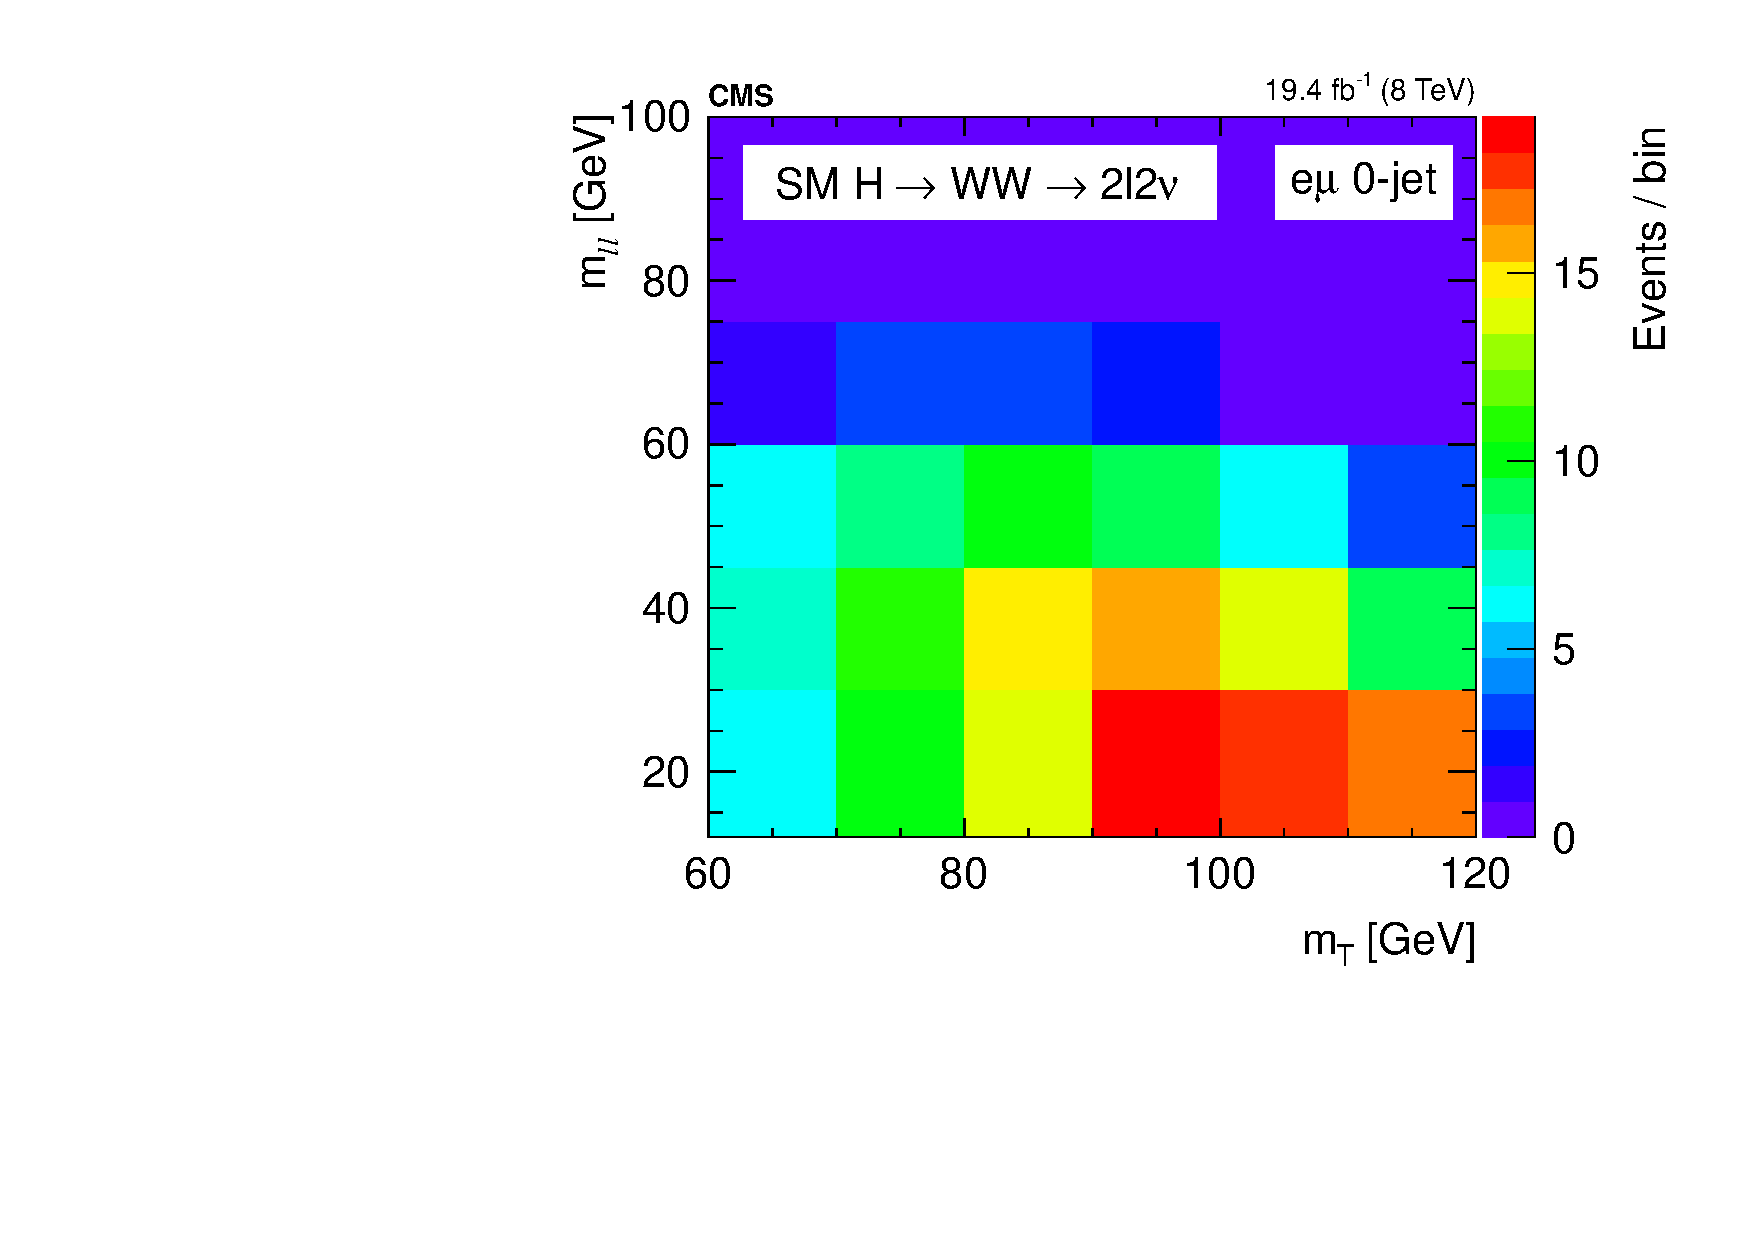
\includegraphics[width=0.45\textwidth]{images/legacyPlots/2d_prefit_0j_125_sig_paper.pdf}}
\subfigure[]{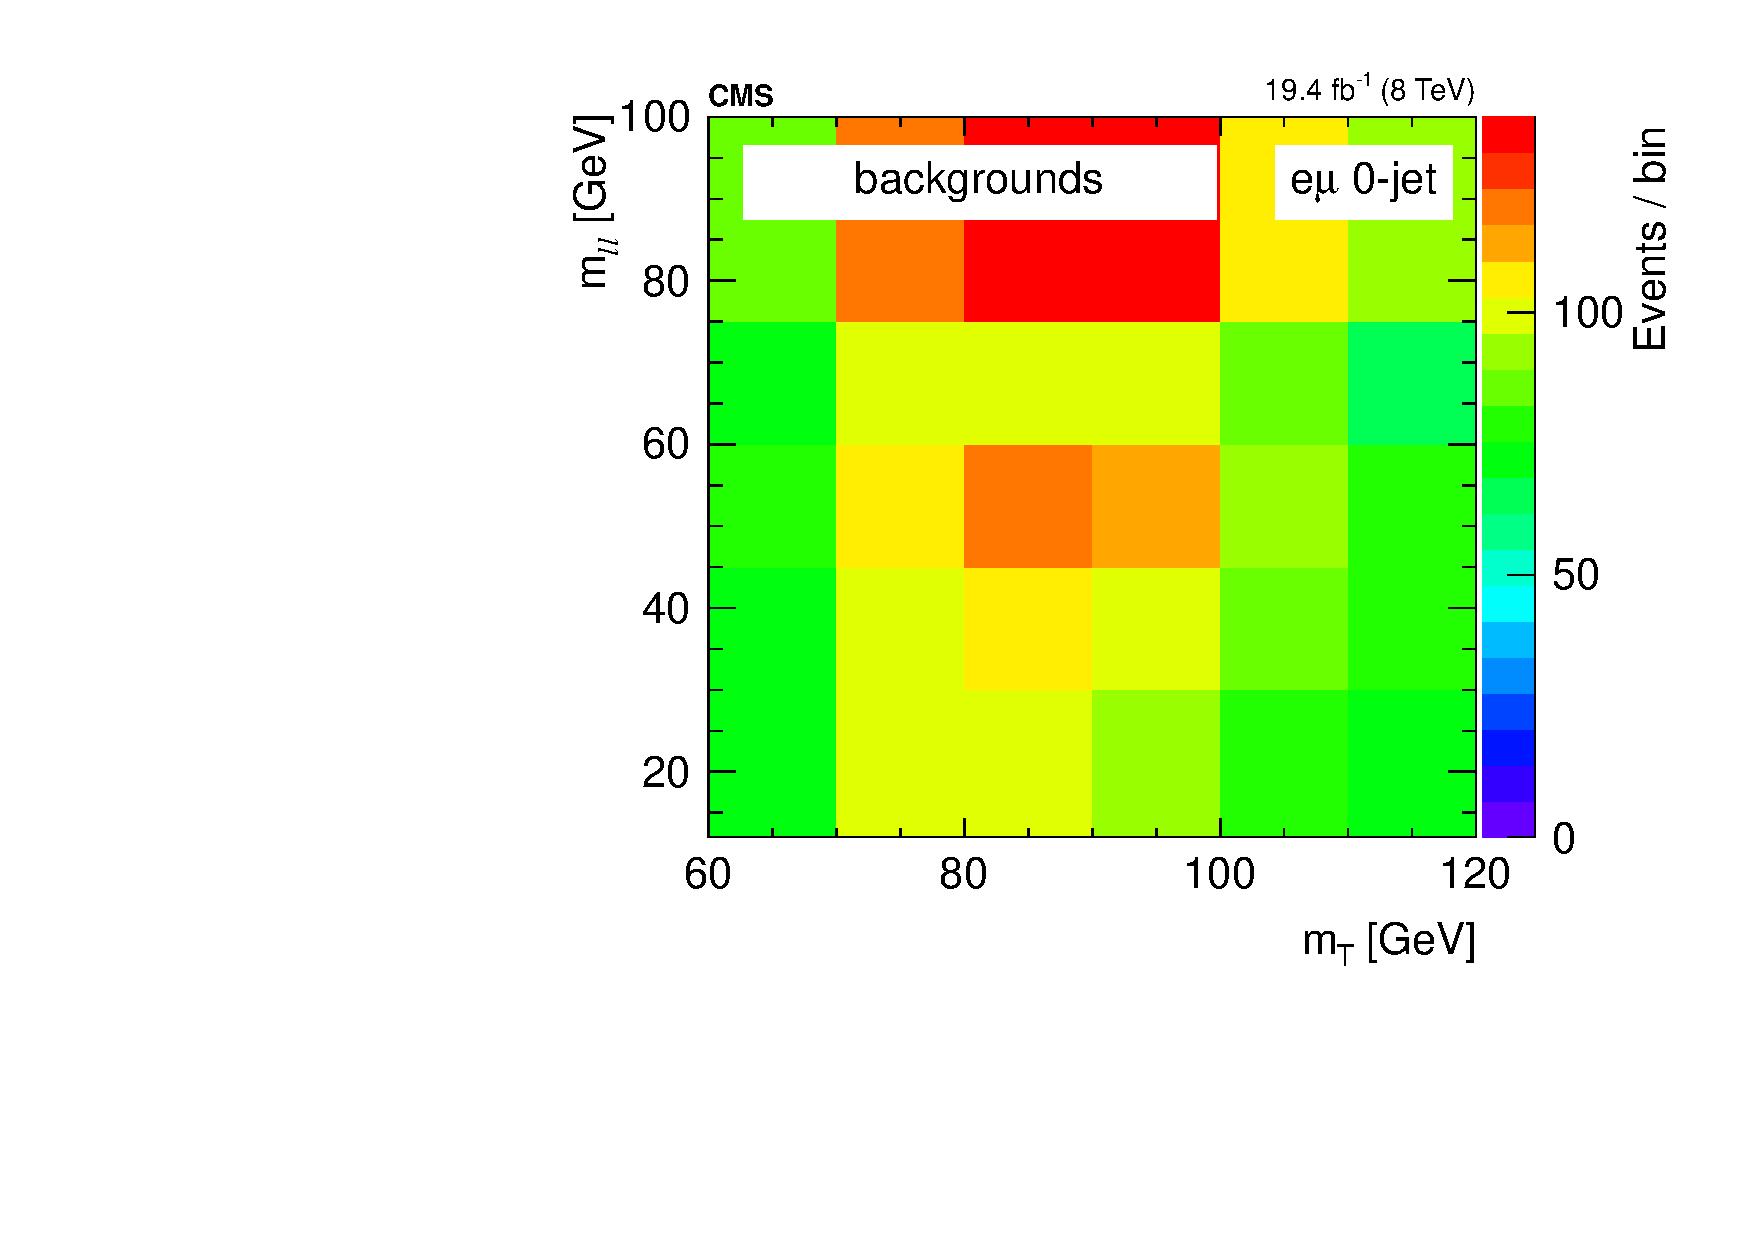
\includegraphics[width=0.45\textwidth]{images/legacyPlots/2d_prefit_0j_125_bkg_paper.pdf}}
\caption{Two-dimensional \mll--\mt distribution for signal (a) and background (b) processes in the 0-jets category.\label{fig:2Dlegacy}}
\end{figure}

Six different signal strength parameters are extracted from the fit, one for each \pth~bin. The relative contributions of the different Higgs production mechanisms in the signal template are taken to be the same as in the SM. The systematic uncertainty sources are considered as nuisance parameters in the fit.

The binning of the \mll and \mt templates is chosen to be:
\begin{itemize}
\item {\mll: $[12,30,45,60,75,100,125,150,175,200]$} 
\item {\mt: $[60,70,80,90,100,110,120,140,160,180,200,220,240,280]$}
\end{itemize}

To avoid a dependence of the results on the variables used for the template fit, \mll and \mt need to be uncorrelated with respect to \pth.
This as been verified and the correlation between the discriminating variables and \pth is shown in Fig.~\ref{fig:correlation_ggH} and Fig.~\ref{fig:correlation_vbf} for ggH and VBF production modes respectively.

\begin{figure}[htb]
\centering
\subfigure[]{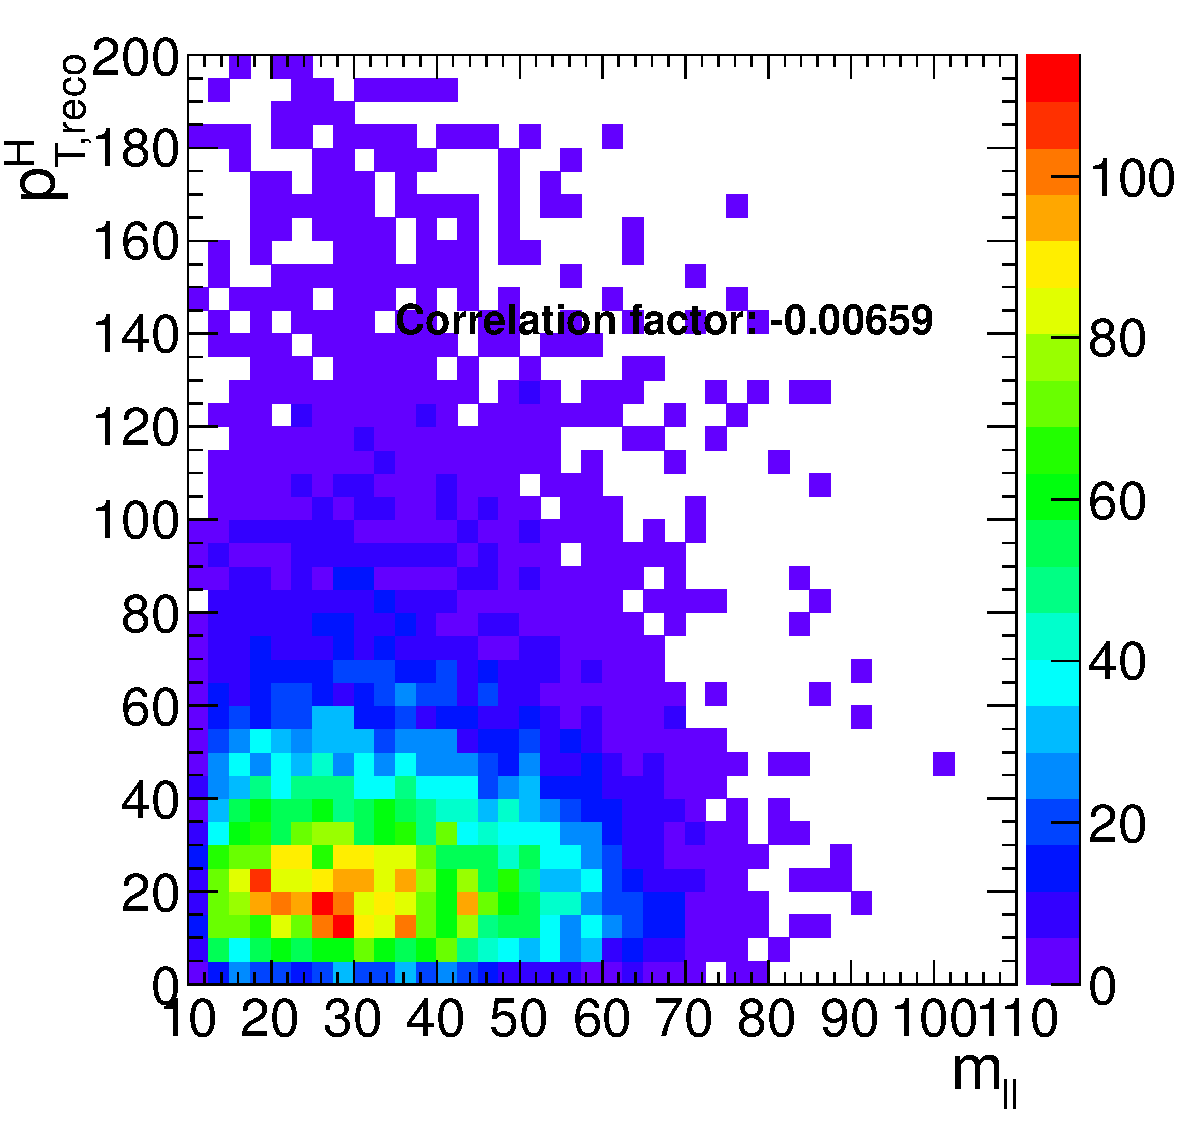
\includegraphics[width=0.45\textwidth]{images/correlationmll_ggH.pdf}}
\subfigure[]{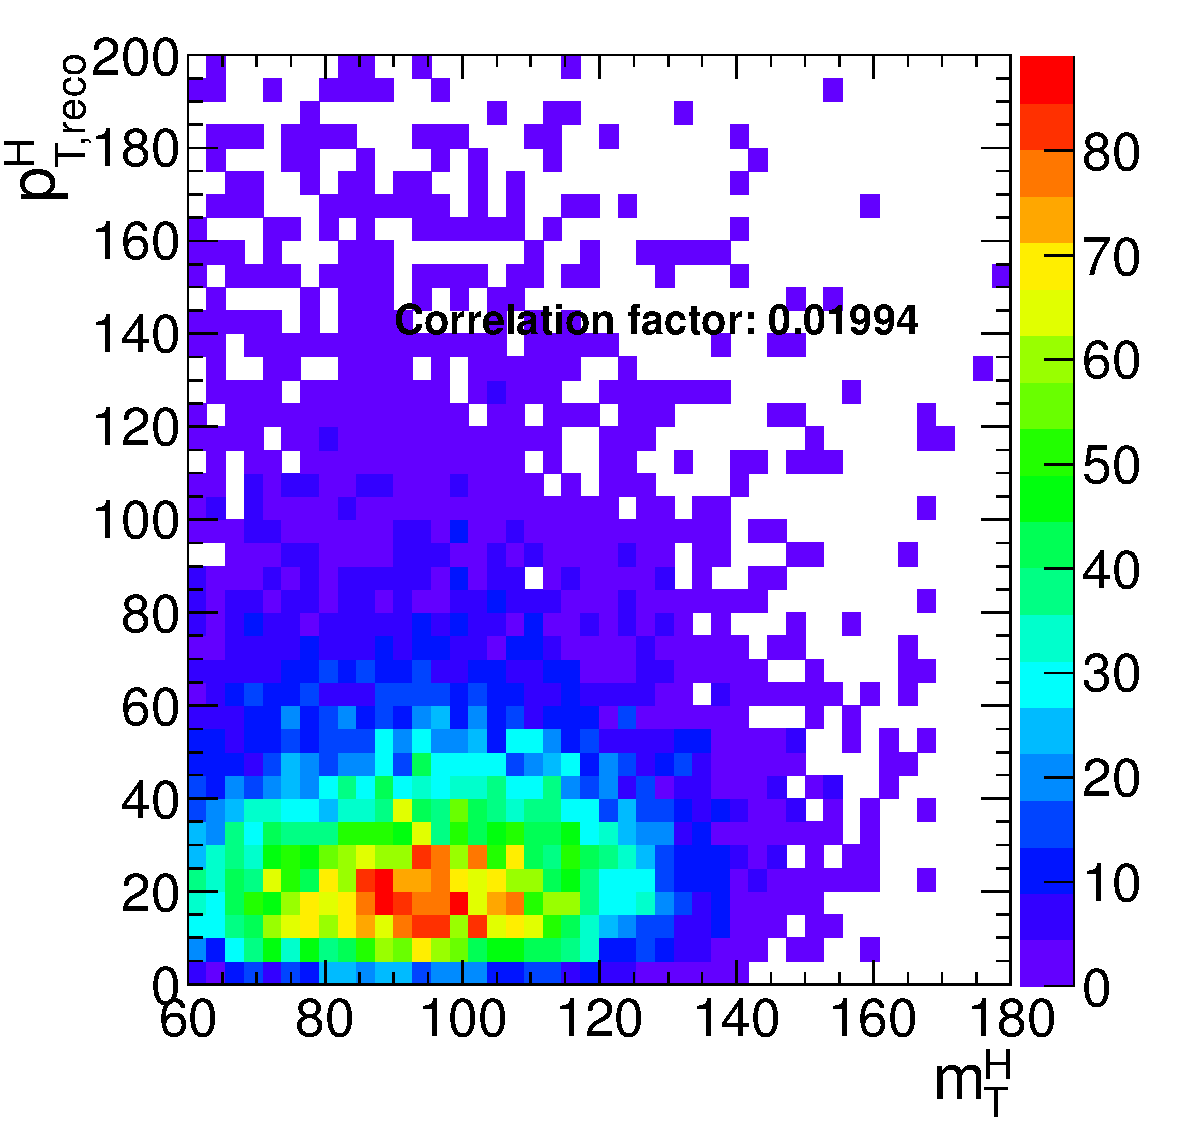
\includegraphics[width=0.45\textwidth]{images/correlationmth_ggH.pdf}}
\caption{Correlation between $\pth$ and $\mll$ (a) and between \pth and \mt (b) after the full selection for the ggH production mode.\label{fig:correlation_ggH}}
\end{figure}

\begin{figure}[htb]
\centering
\subfigure[]{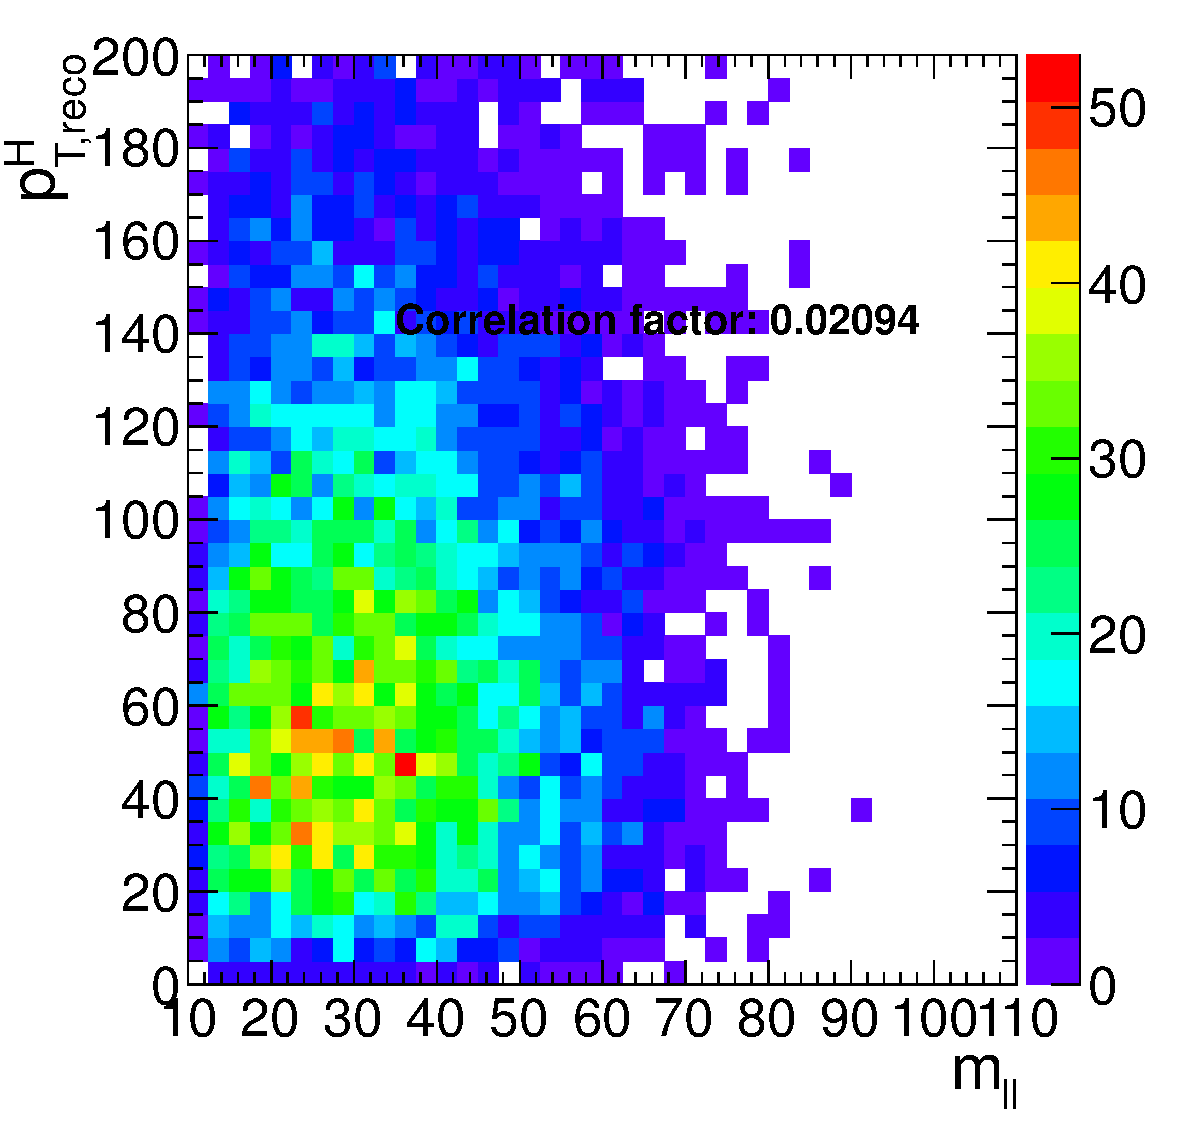
\includegraphics[width=0.45\textwidth]{images/correlationmll_vbf.pdf}}
\subfigure[]{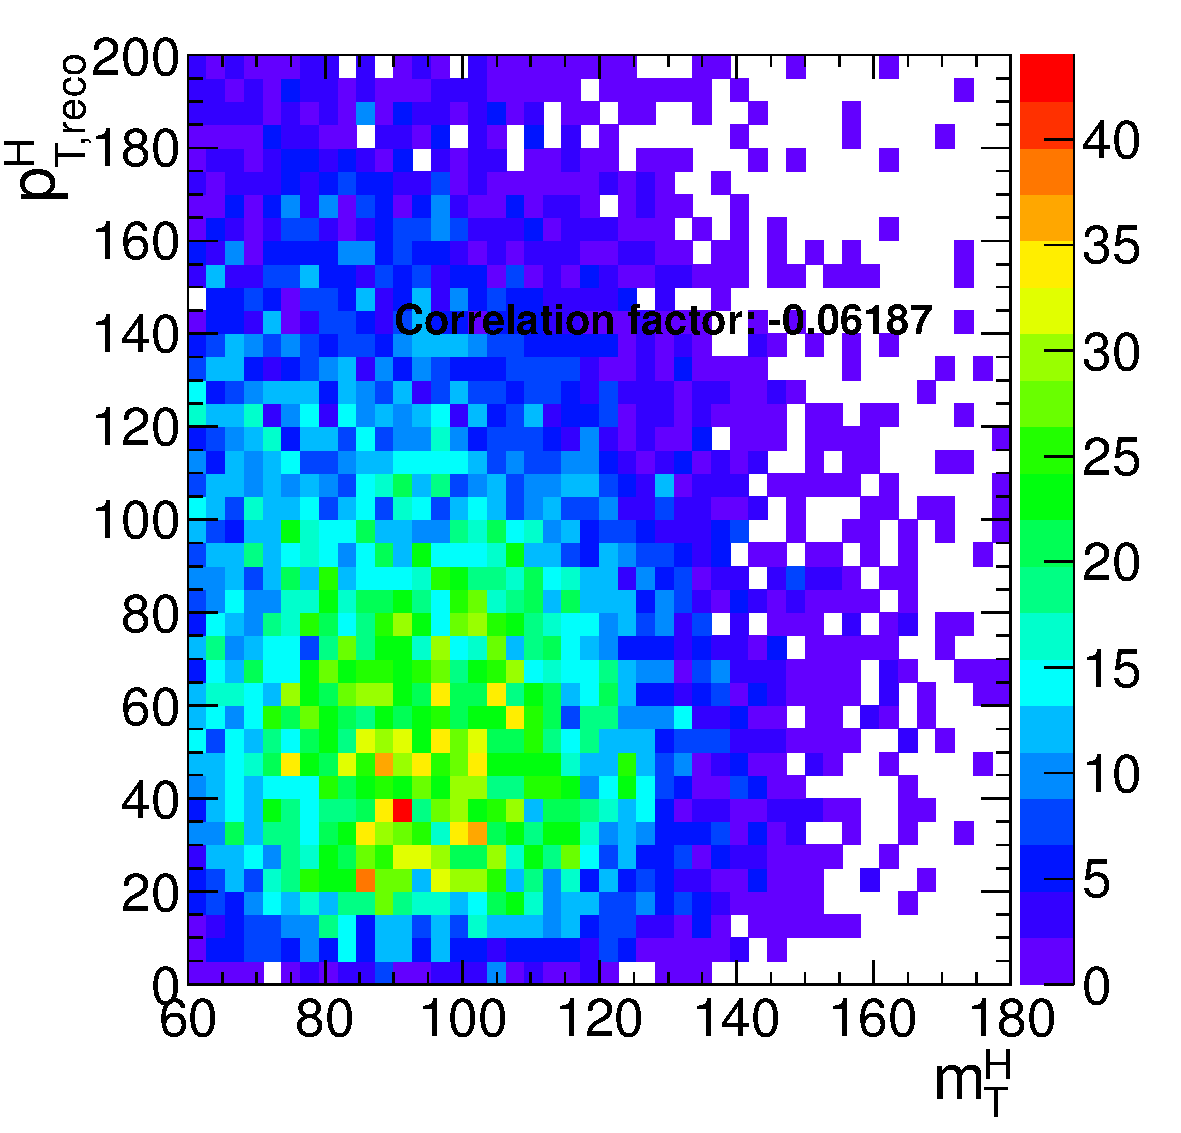
\includegraphics[width=0.45\textwidth]{images/correlationmth_vbf.pdf}}
\caption{Correlation between \pth and \mll (a) and between \pth and \mt (b) after the full selection for the VBF production mode.\label{fig:correlation_vbf}}
\end{figure}

The relative contribution for different production mechanisms in the input signal template is taken to be the same as the SM.
The signal strength $\mu$ in each bin, i.e. the ratio between the measured cross section and the SM one, $\mu = \sigma/\sigma_\mathrm{SM}$, is allowed to float between -10 and +10, thus allowing negative values. This is mainly intended to allow the error bars to float below 0.

Because of detector resolution effects, some of the reconstructed $\hww$ signal events might originate from outside the fiducial phase space.  
These out-of-fiducial signal events cannot be precisely handled by the unfolding procedure and must be subtracted from the measured spectrum. The \pth~distribution of the out-of-fiducial signal events is taken from simulation, and each bin is multiplied by the corresponding measured signal strength before performing the subtraction. 

At the end, the number of events in each bin $i$ of the measured spectrum is:
\begin{equation}
N_i = \mu_i (s_i -f_i) \quad ,
\end{equation}
where $s_i$ and $f_i$ are respectively the number of signal and fake events expected from simulation and $\mu_i$ is the measured signal strength.

The fit makes use of the binned maximum likelihood approach. Each source of systematic uncertainty is represented by a nuisance parameter in the likelihood function. \textcolor{red}{add some techincality about the fit, i.e. different priors of the nuisance parameters etc.}

Before running the fit on the data, the same procedure has been applied on the so called \textit{Asimov data set}\footnote{In a parallel reality imagined by the science fiction writer I. Asimov, politics was run in a peculiar way: instead of mobilizing millions of people to cast their vote to deliberate on something, an algorithm was used to select an individual ``average'' person, and then this person was asked to take the decision on that matter.}, which provides a simple method to obtain the signal sensitivity before looking at the data~\cite{Cowan:2010js}.


\subsection{Signal and background yields}\label{subsec:yields}


A comparison of data and background prediction is shown in
Fig.~\ref{fig:mllSignalRegion}, where the \mll{} distribution is shown for the six \pth{} bins. Distributions correspond to the \mt{} window of [60, 110]\GeV, in order to emphasize the signal contribution~\cite{Chatrchyan:2013iaa}. The \mt distributions are shown in Fig.~\ref{fig:mTSignalRegion} and correspond to the \mll window of [12, 75]\GeV.

\begin{figure}[!htbp]
\centering
\subfigure{
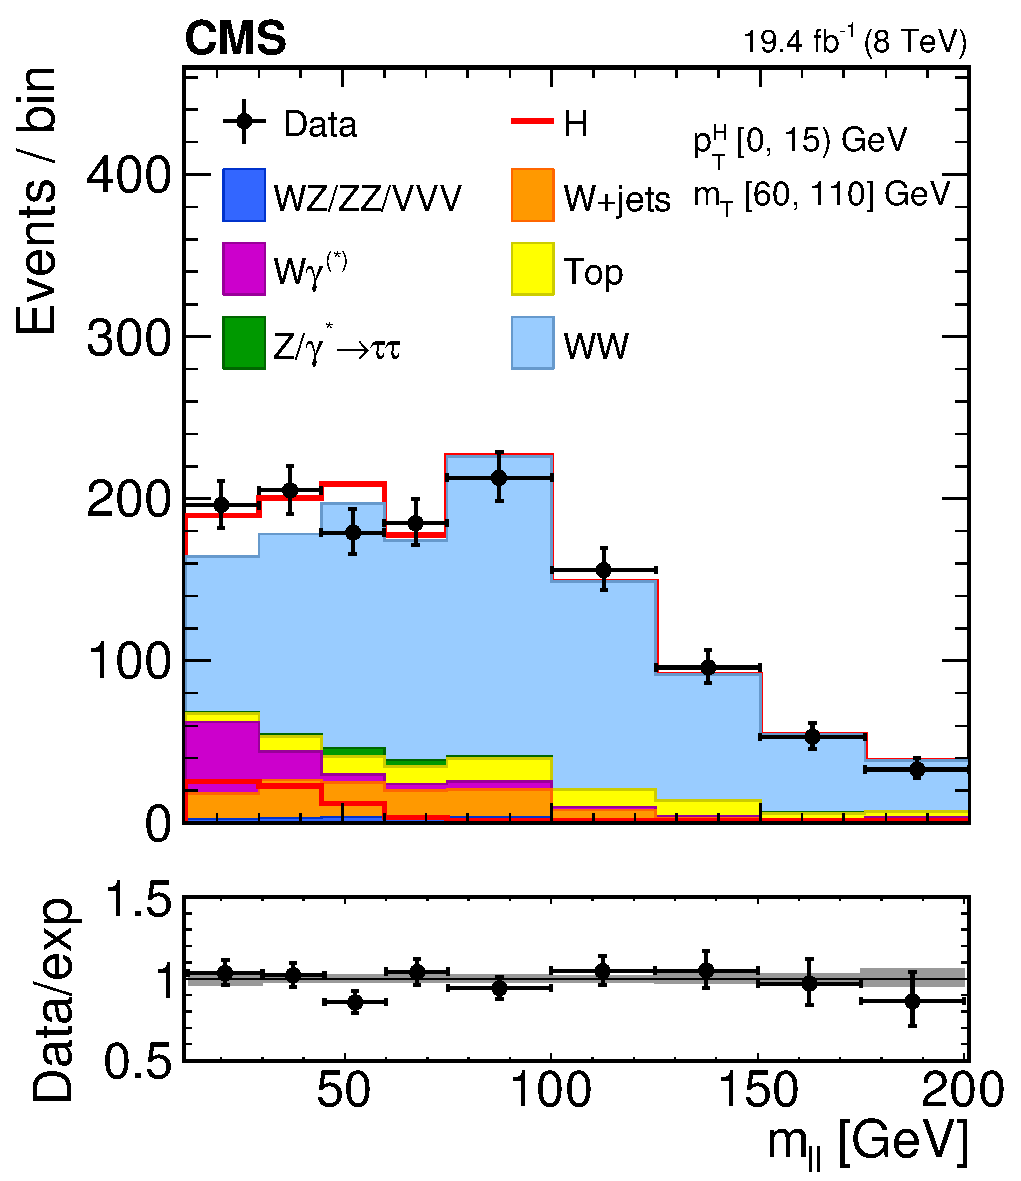
\includegraphics[width=0.31\textwidth]{images/unblinding/mllBin0.pdf}
}
\subfigure{
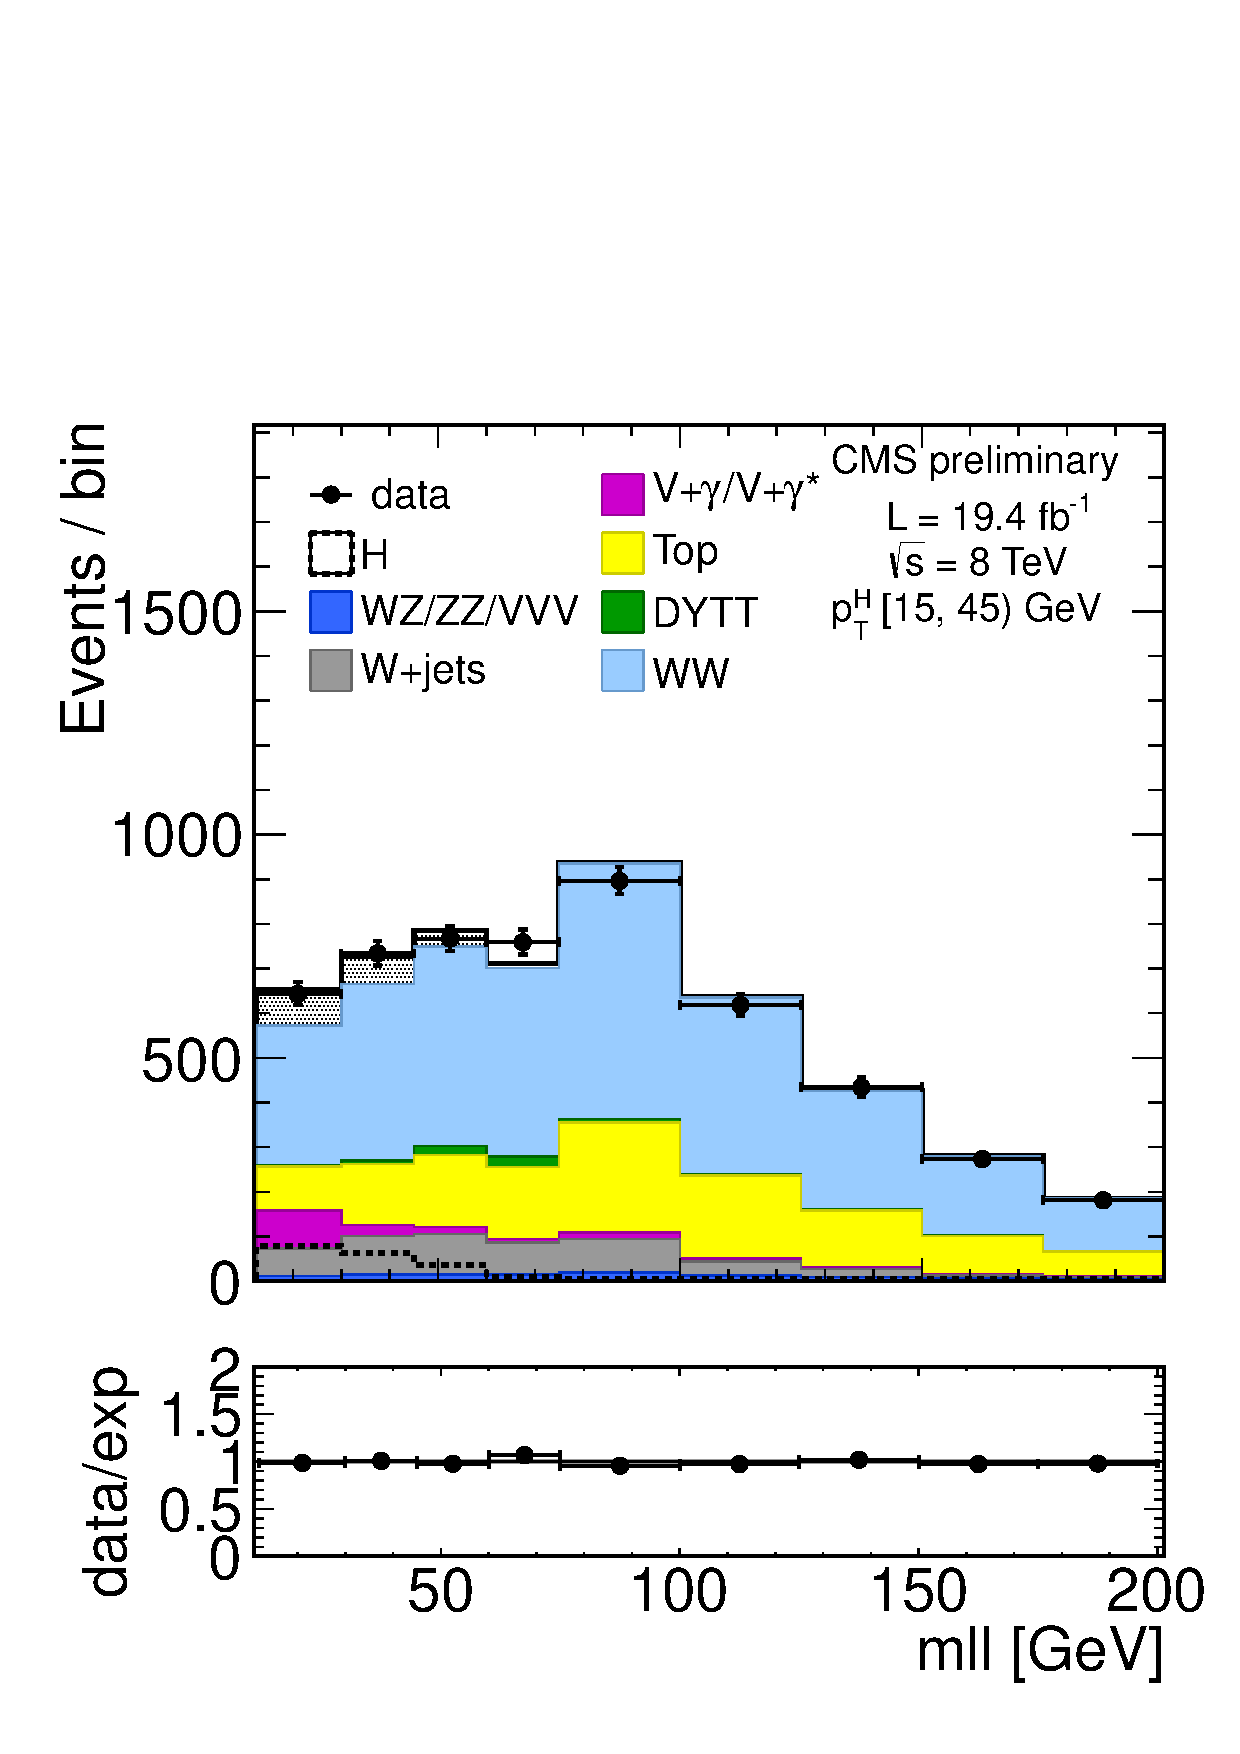
\includegraphics[width=0.31\textwidth]{images/unblinding/mllBin1.pdf}
}
\subfigure{
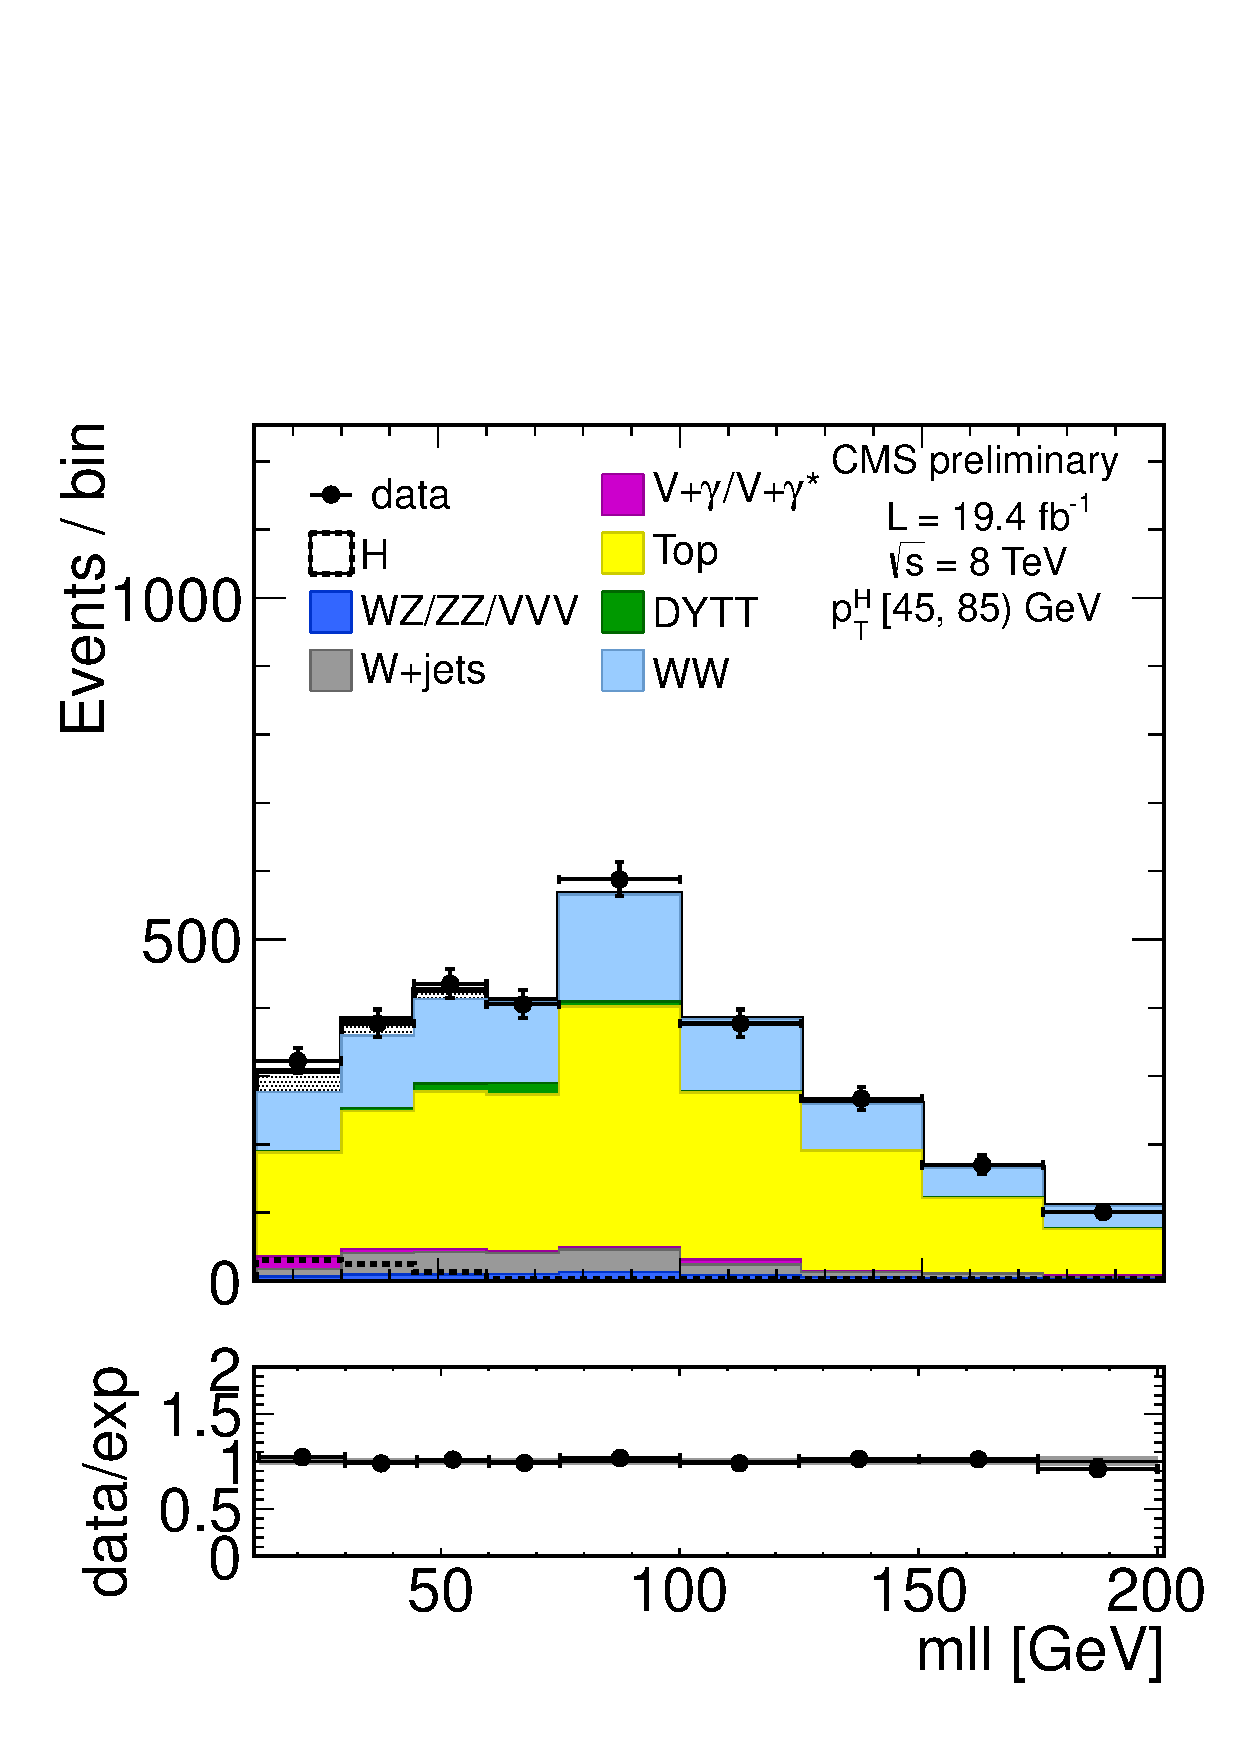
\includegraphics[width=0.31\textwidth]{images/unblinding/mllBin2.pdf}
}
\subfigure{
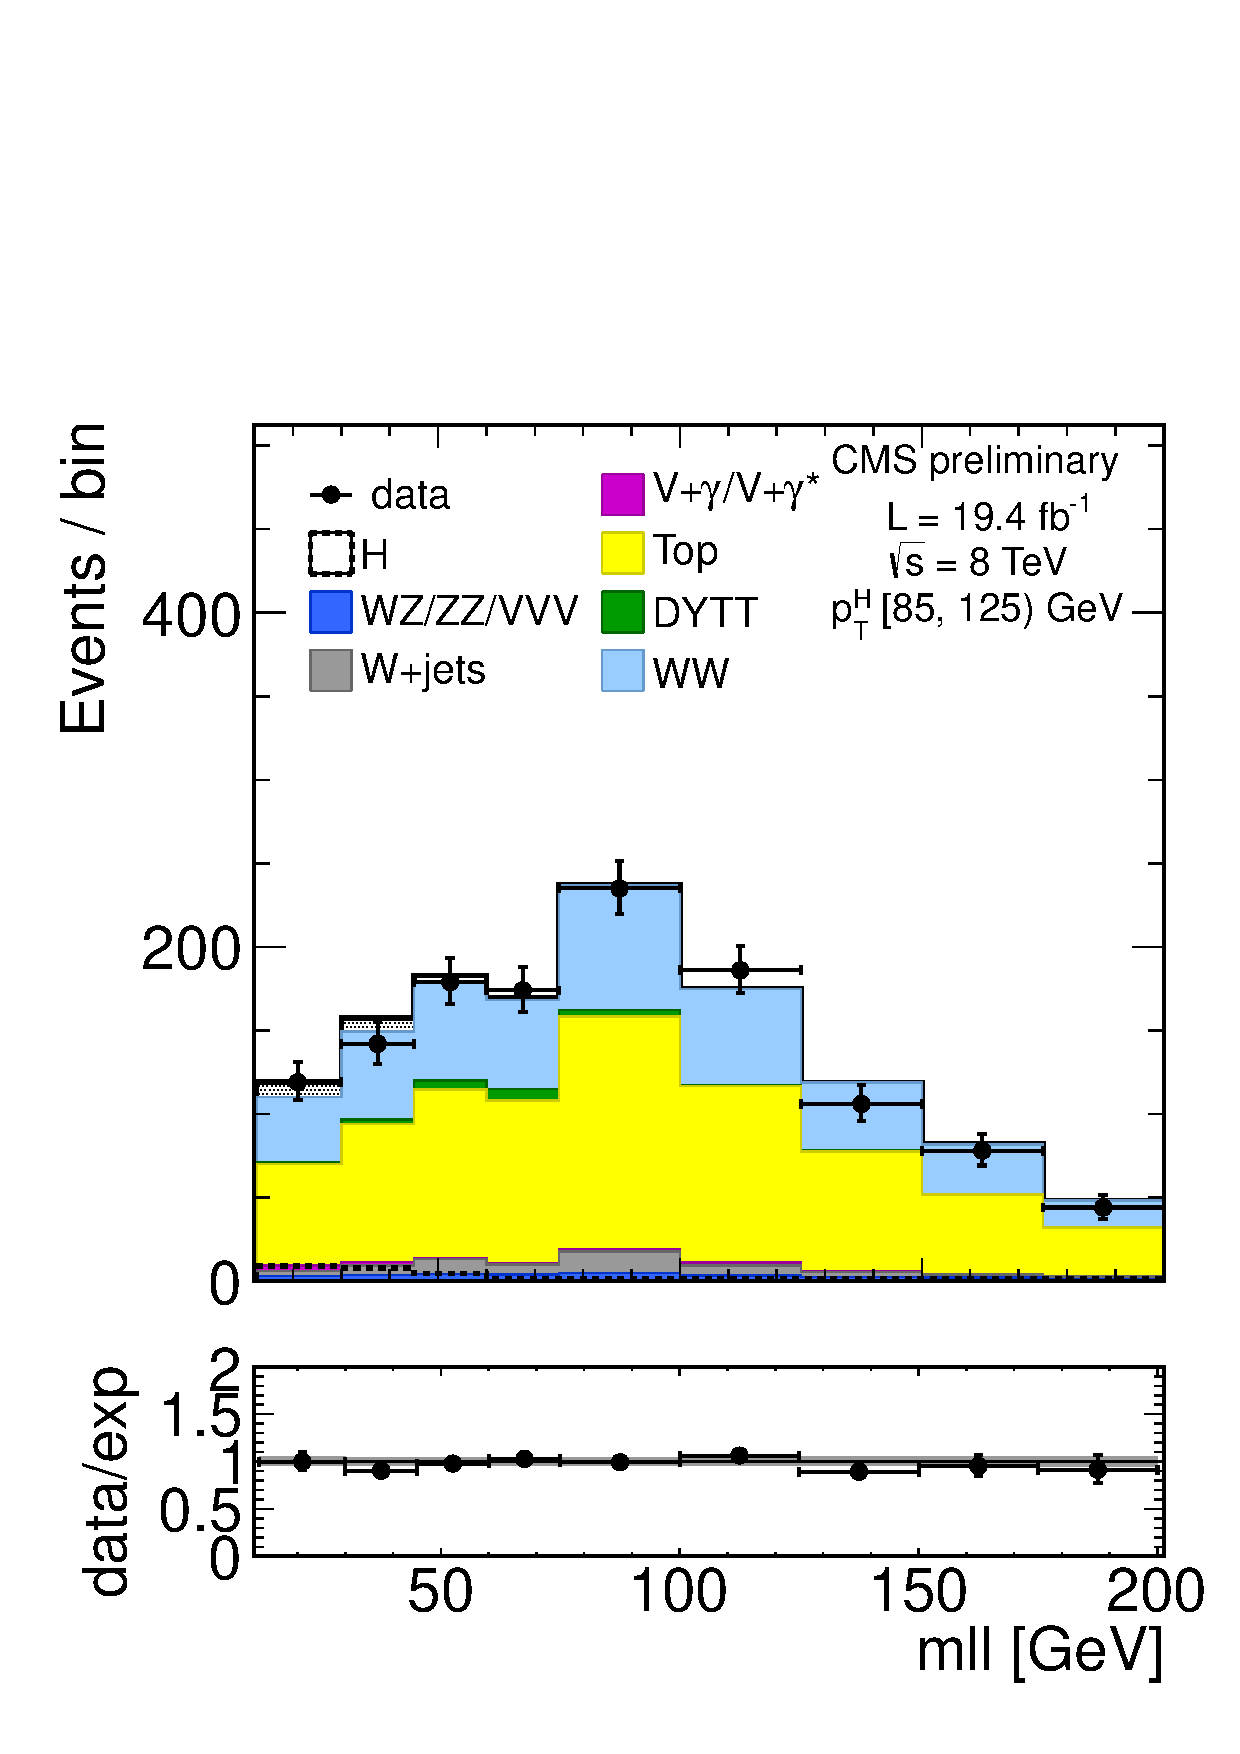
\includegraphics[width=0.31\textwidth]{images/unblinding/mllBin3.pdf}
}
\subfigure{
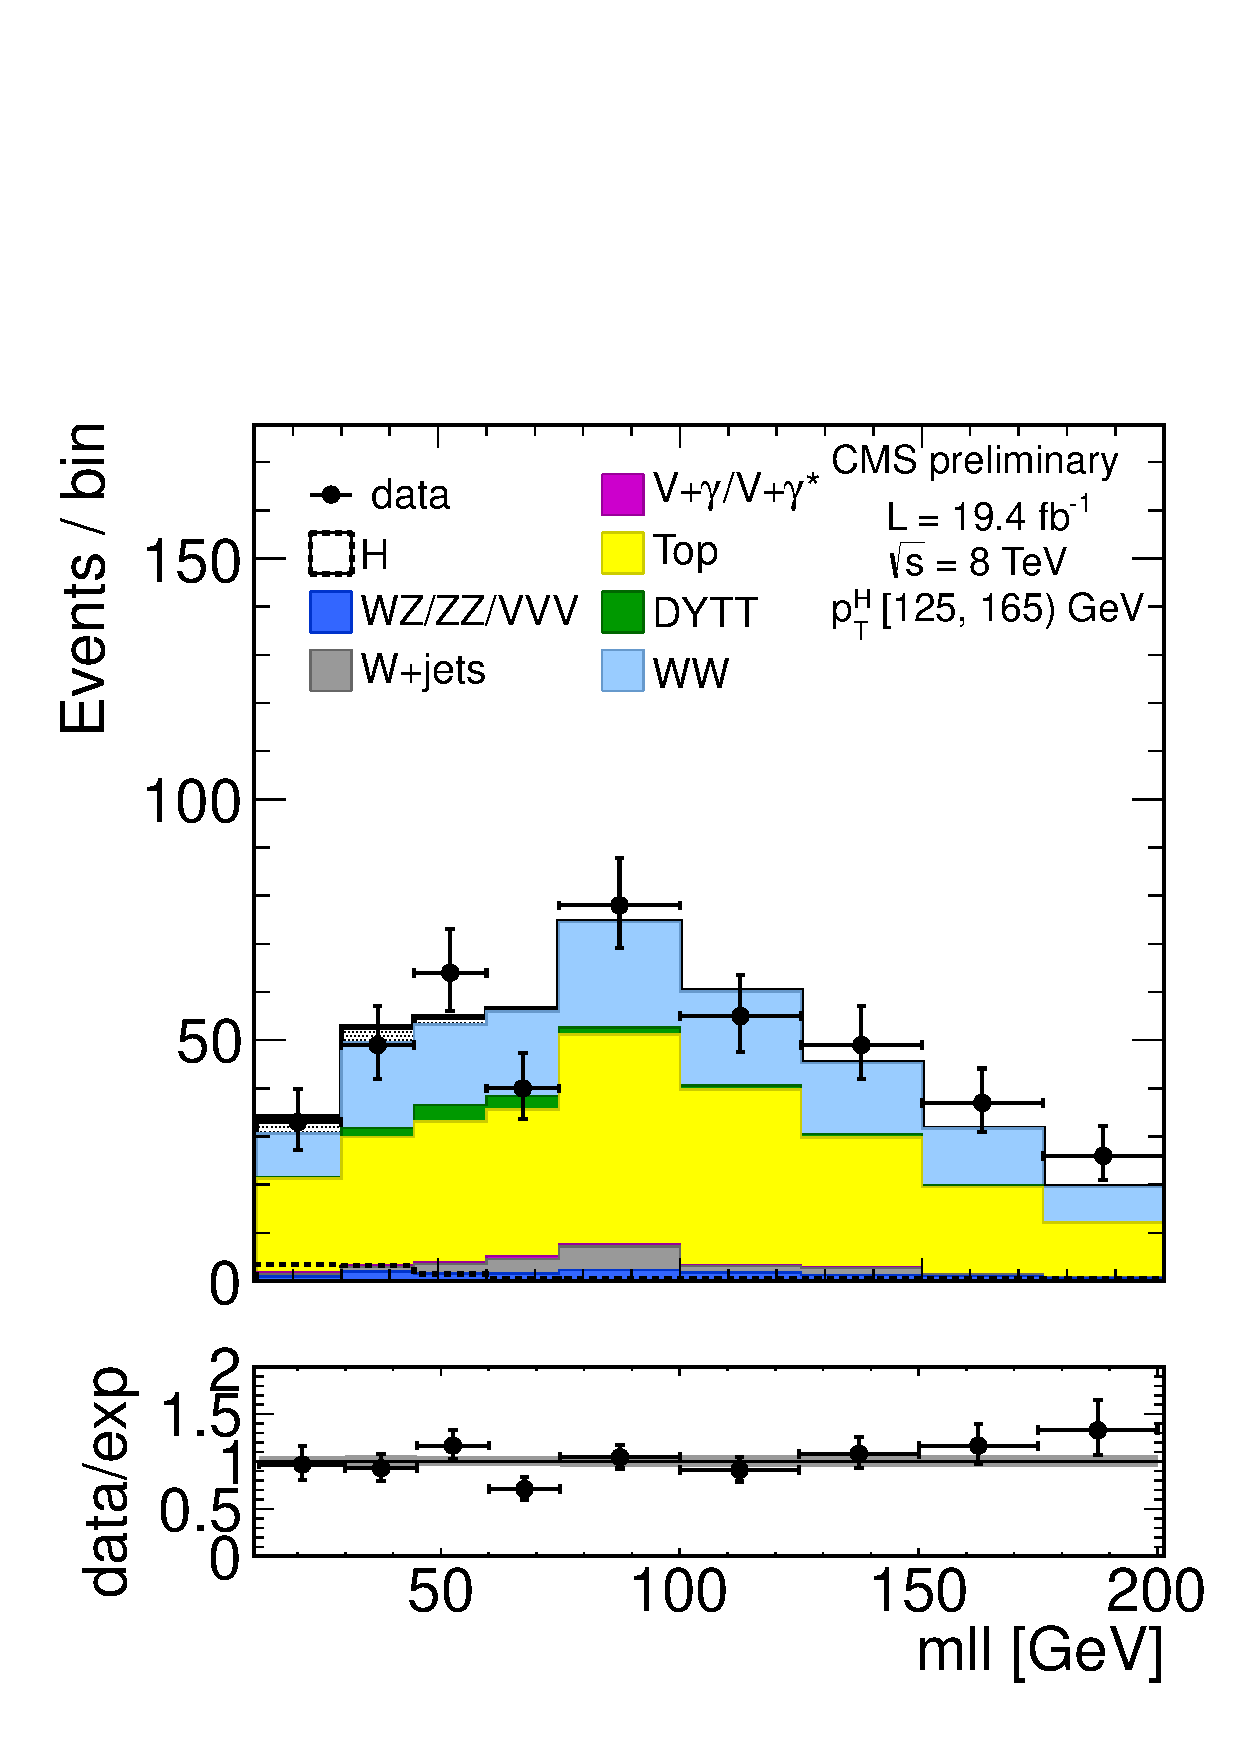
\includegraphics[width=0.31\textwidth]{images/unblinding/mllBin4.pdf}
}
\subfigure{
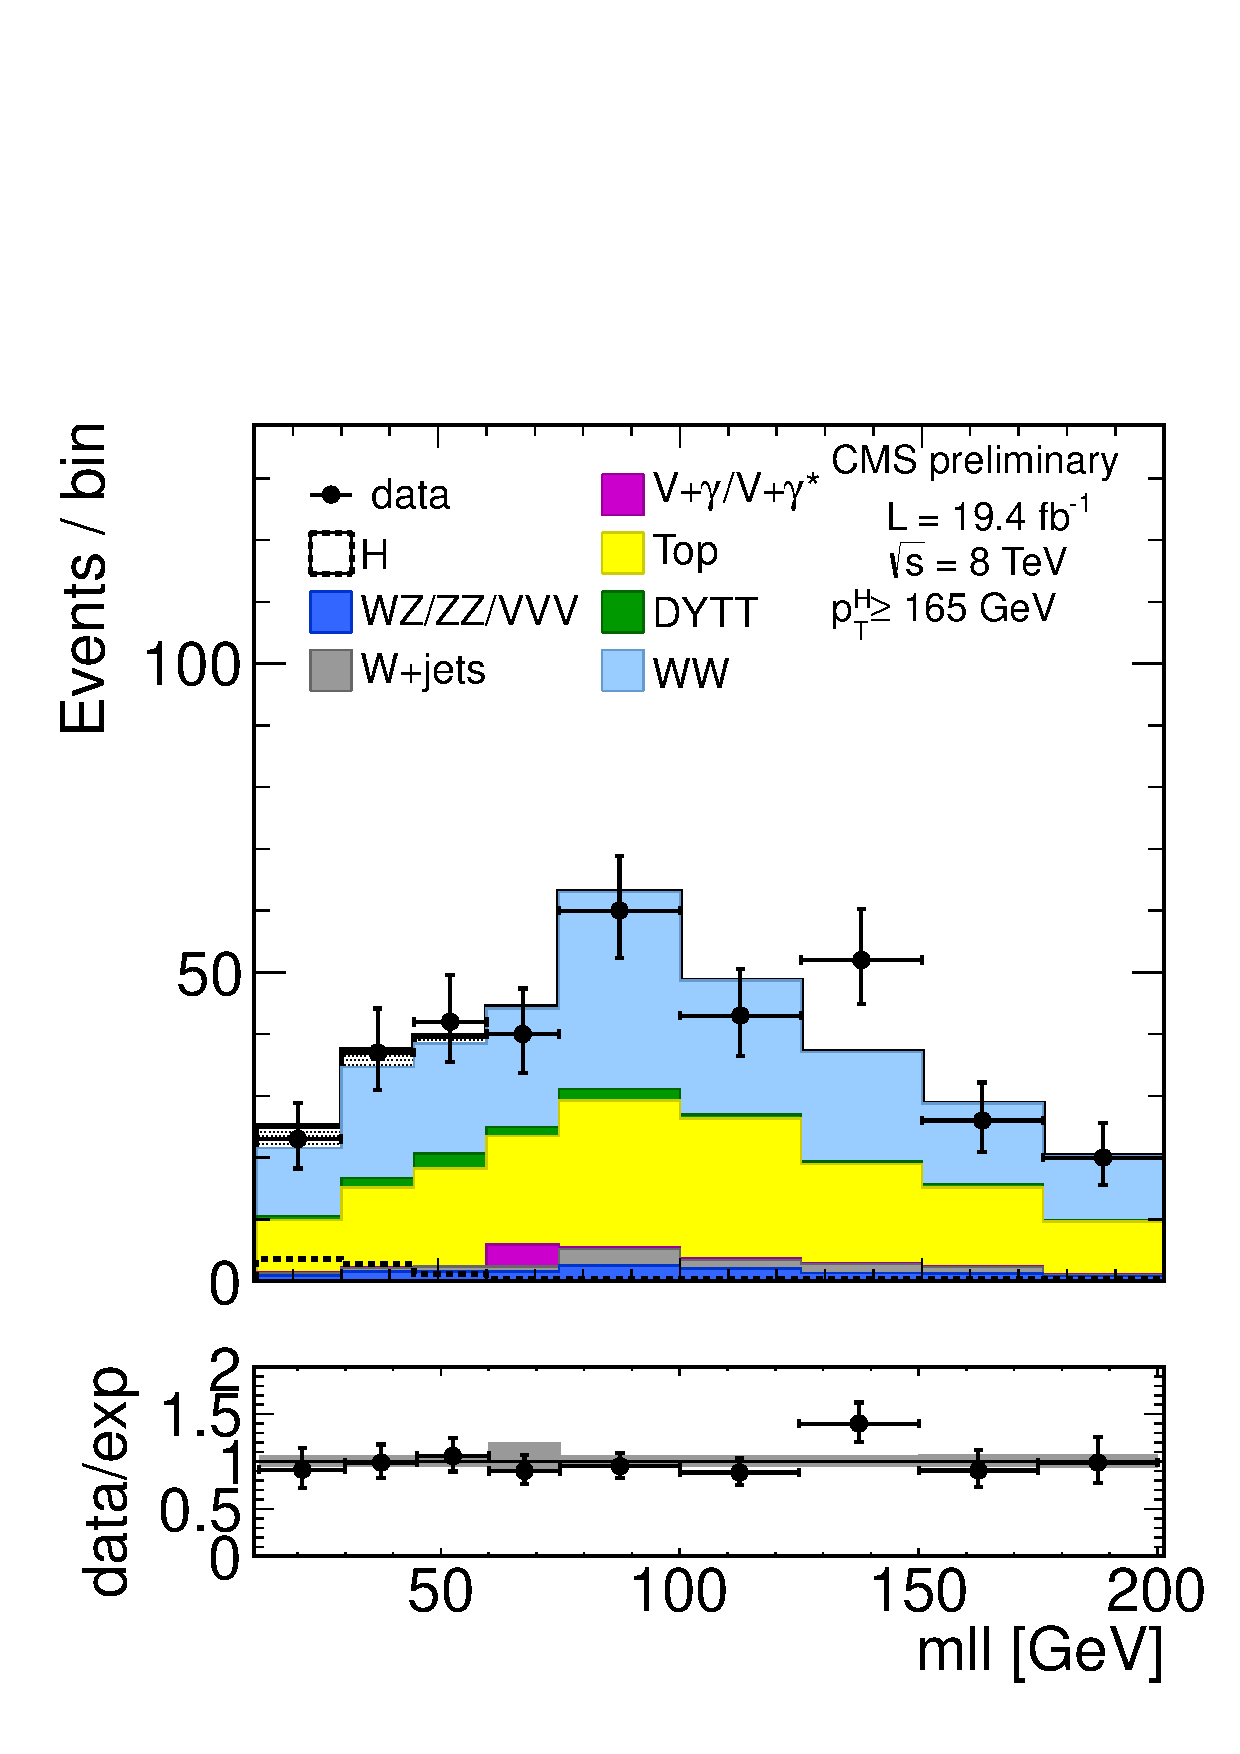
\includegraphics[width=0.31\textwidth]{images/unblinding/mllBin5.pdf}
}
\caption{Distributions of the \mll~variable in each of the six \pth{} bins. Background normalizations correspond to the values obtained from the fit. Signal normalization is fixed to the SM expectation. The distributions are shown in an \mt{}~window of [60,110]\GeV in order to emphasize the Higgs boson (H) signal. The signal contribution is shown both stacked on top of the background and superimposed to it. Ratios of the expected and observed event yields in individual bins are shown in the panels below the plots. The uncertainty band shown in the ratio plot corresponds to the envelope of systematic uncertainties after performing the fit to the data.}\label{fig:mllSignalRegion}
\end{figure}

\begin{figure}[!htbp]
\centering
\subfigure{
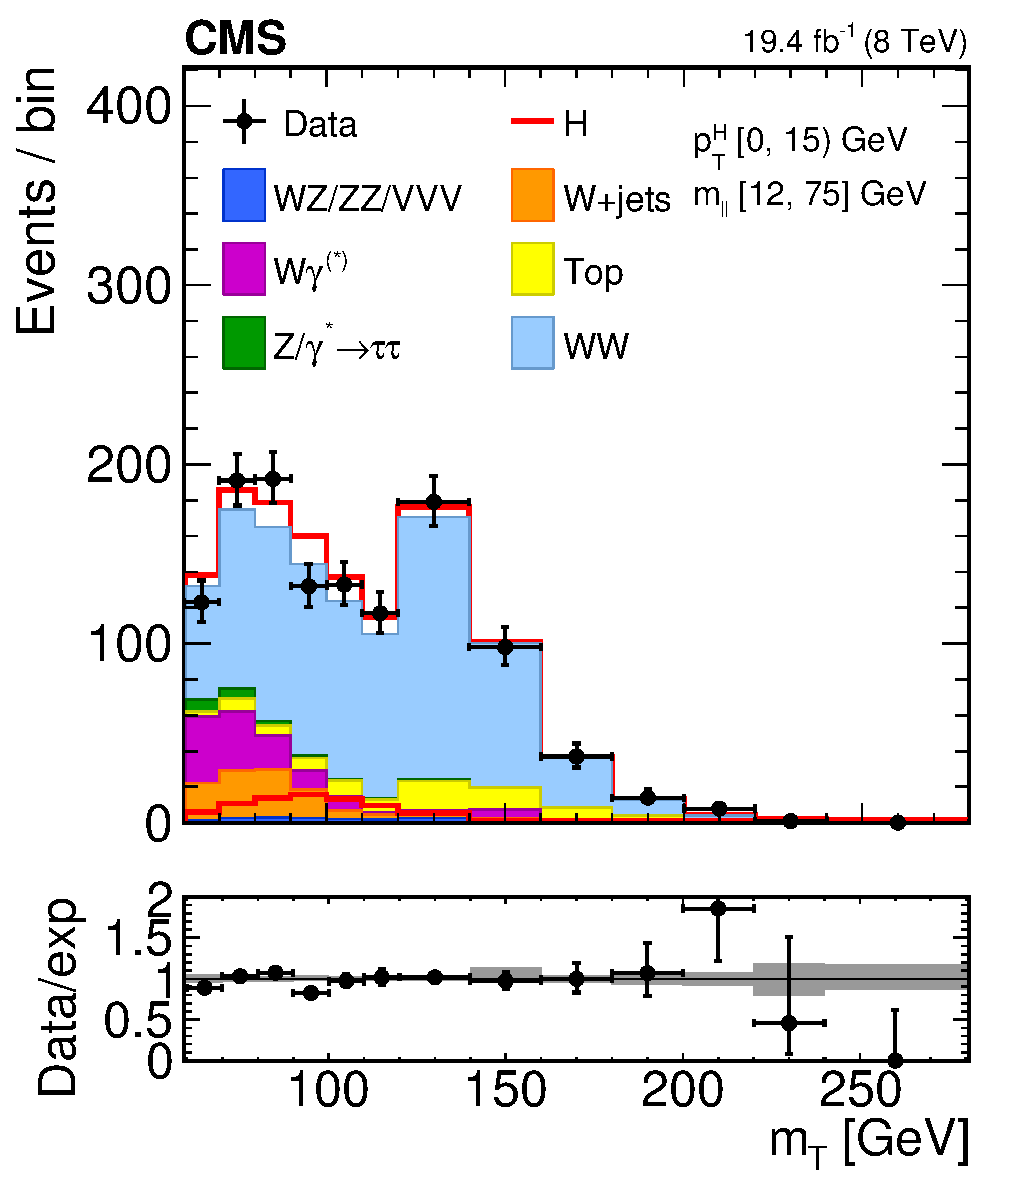
\includegraphics[width=0.31\textwidth]{images/unblinding/mTBin0.pdf}
}
\subfigure{
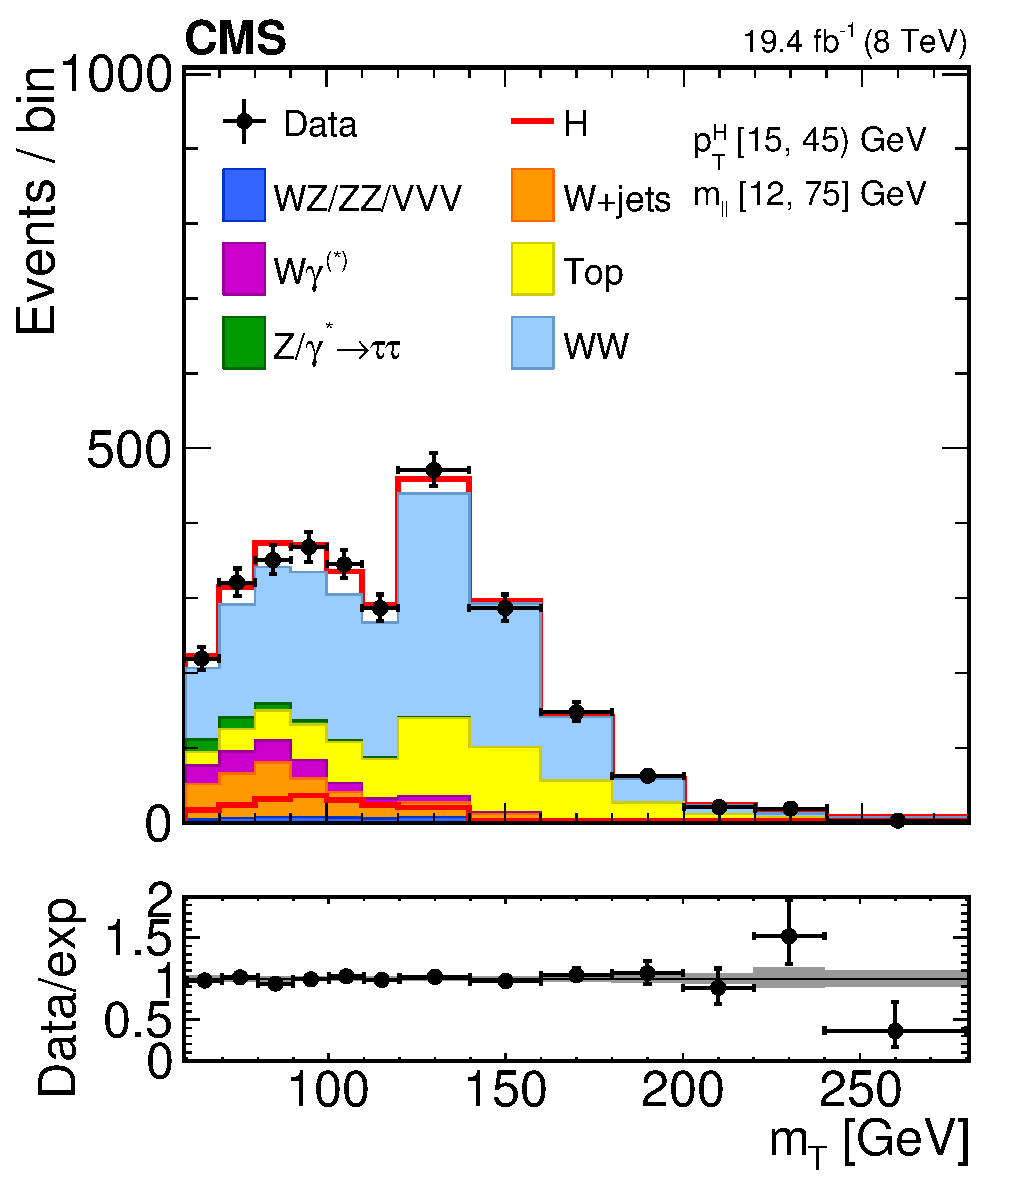
\includegraphics[width=0.31\textwidth]{images/unblinding/mTBin1.pdf}
}
\subfigure{
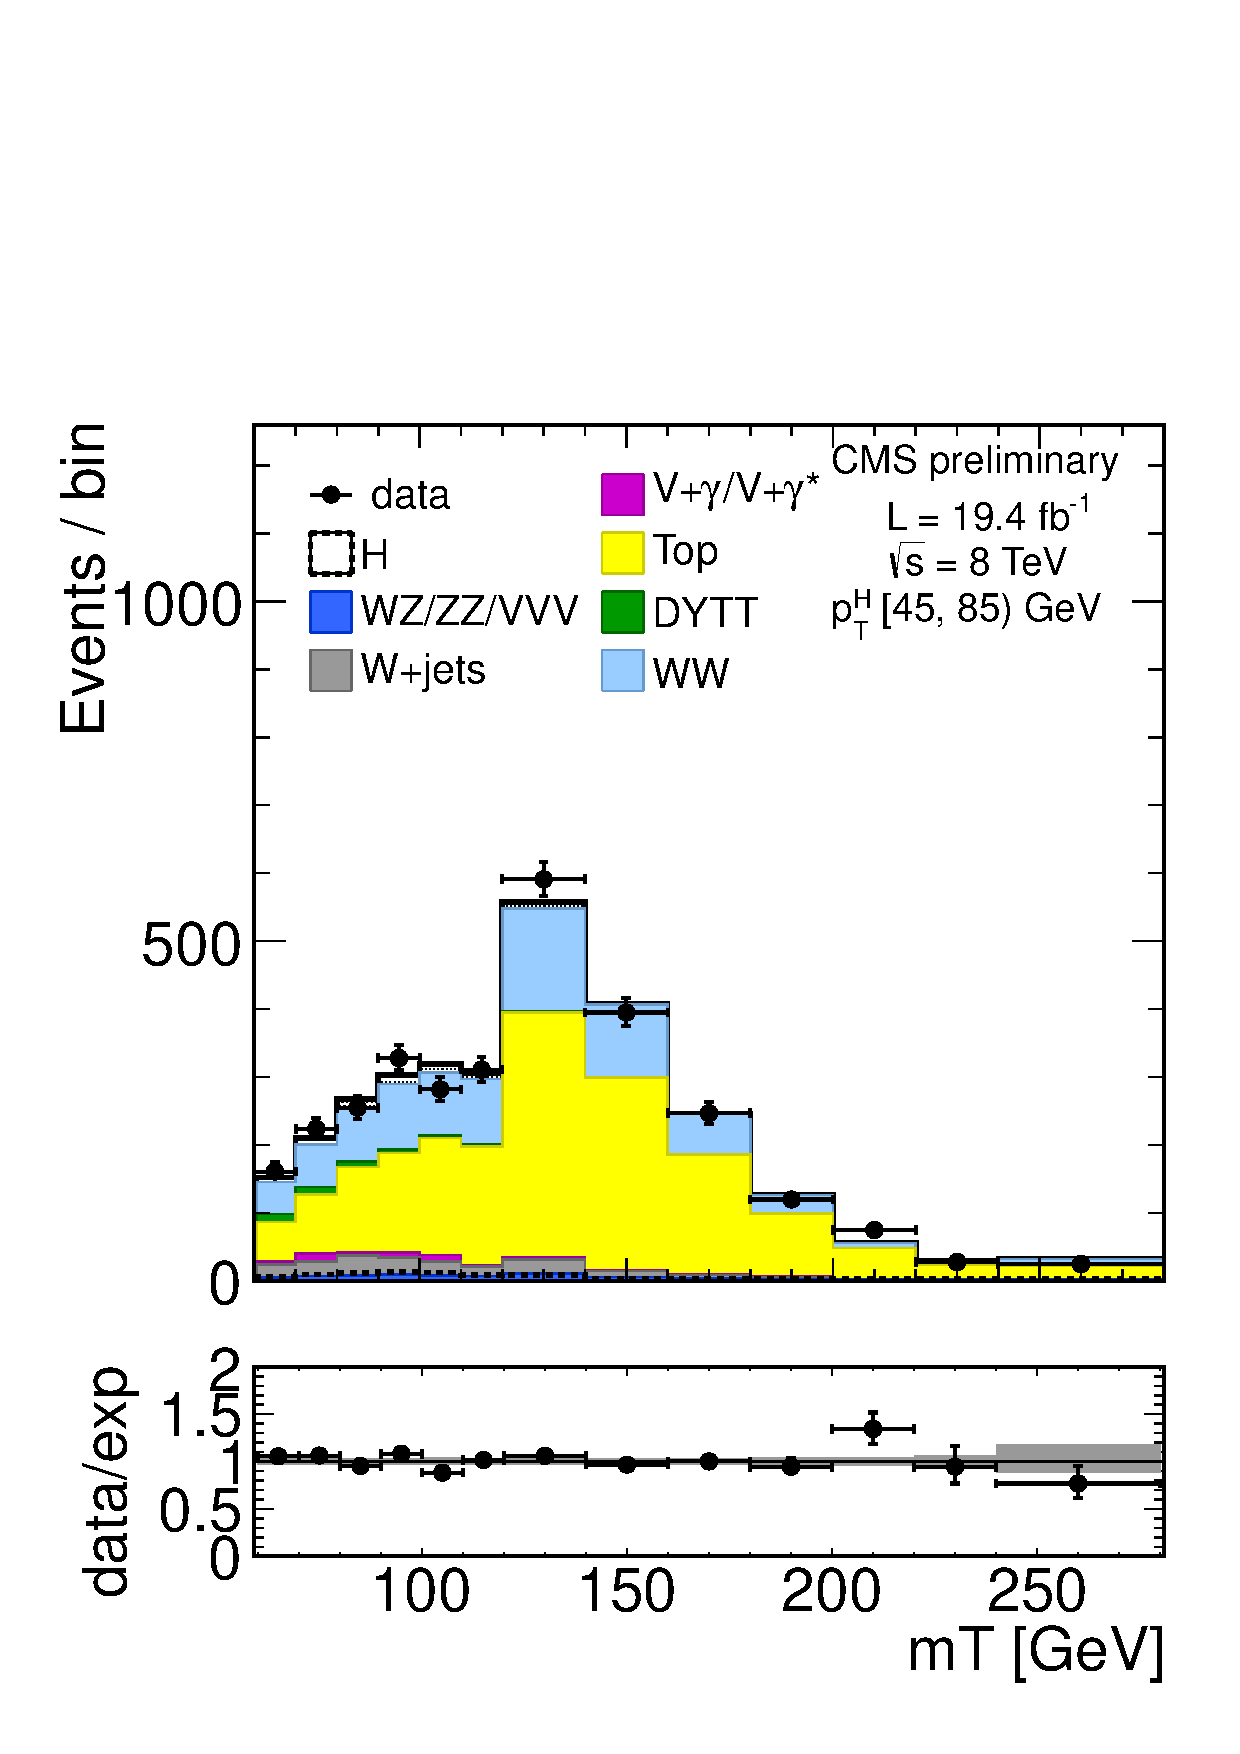
\includegraphics[width=0.31\textwidth]{images/unblinding/mTBin2.pdf}
}
\subfigure{
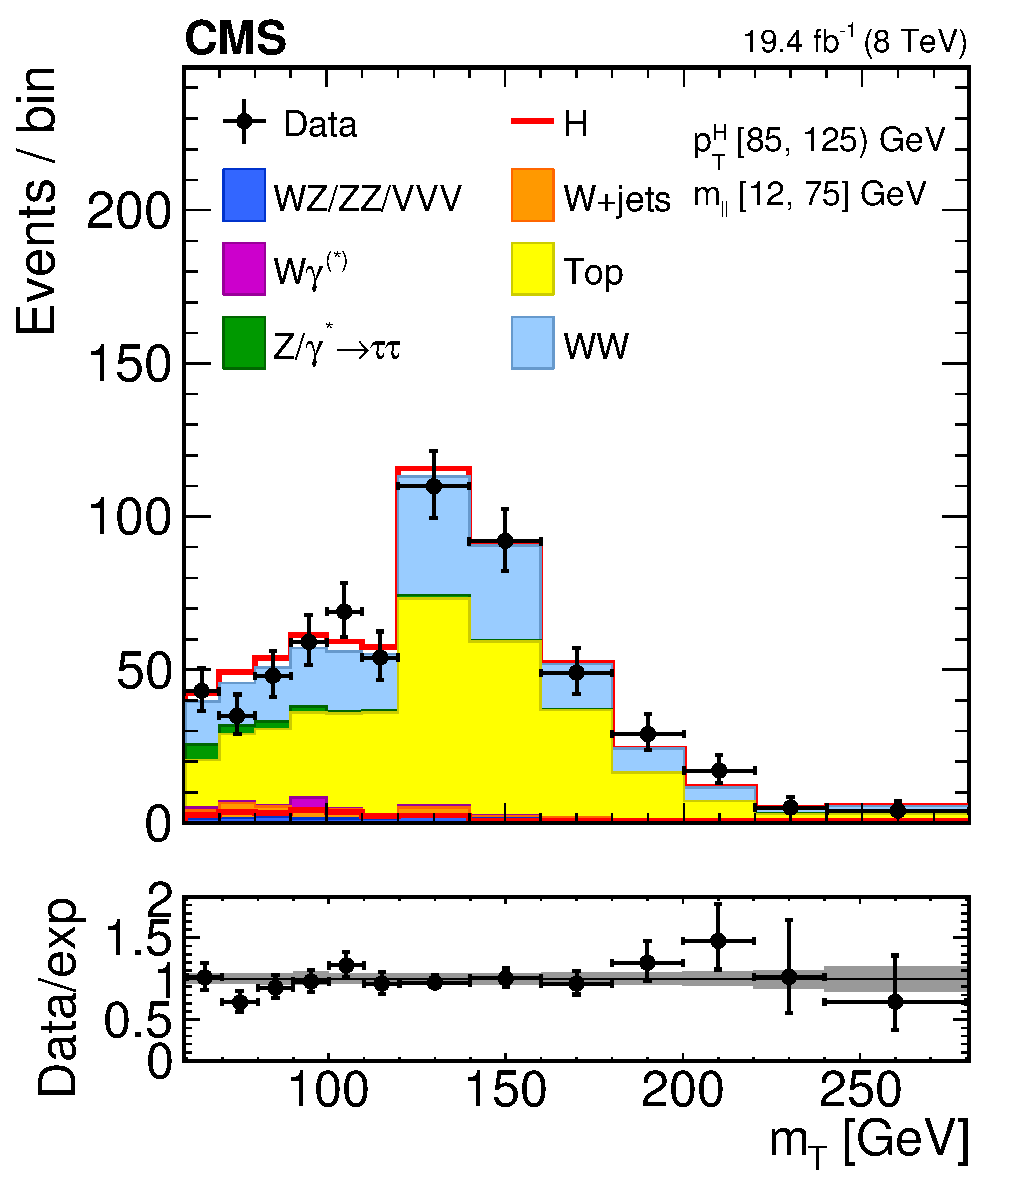
\includegraphics[width=0.31\textwidth]{images/unblinding/mTBin3.pdf}
}
\subfigure{
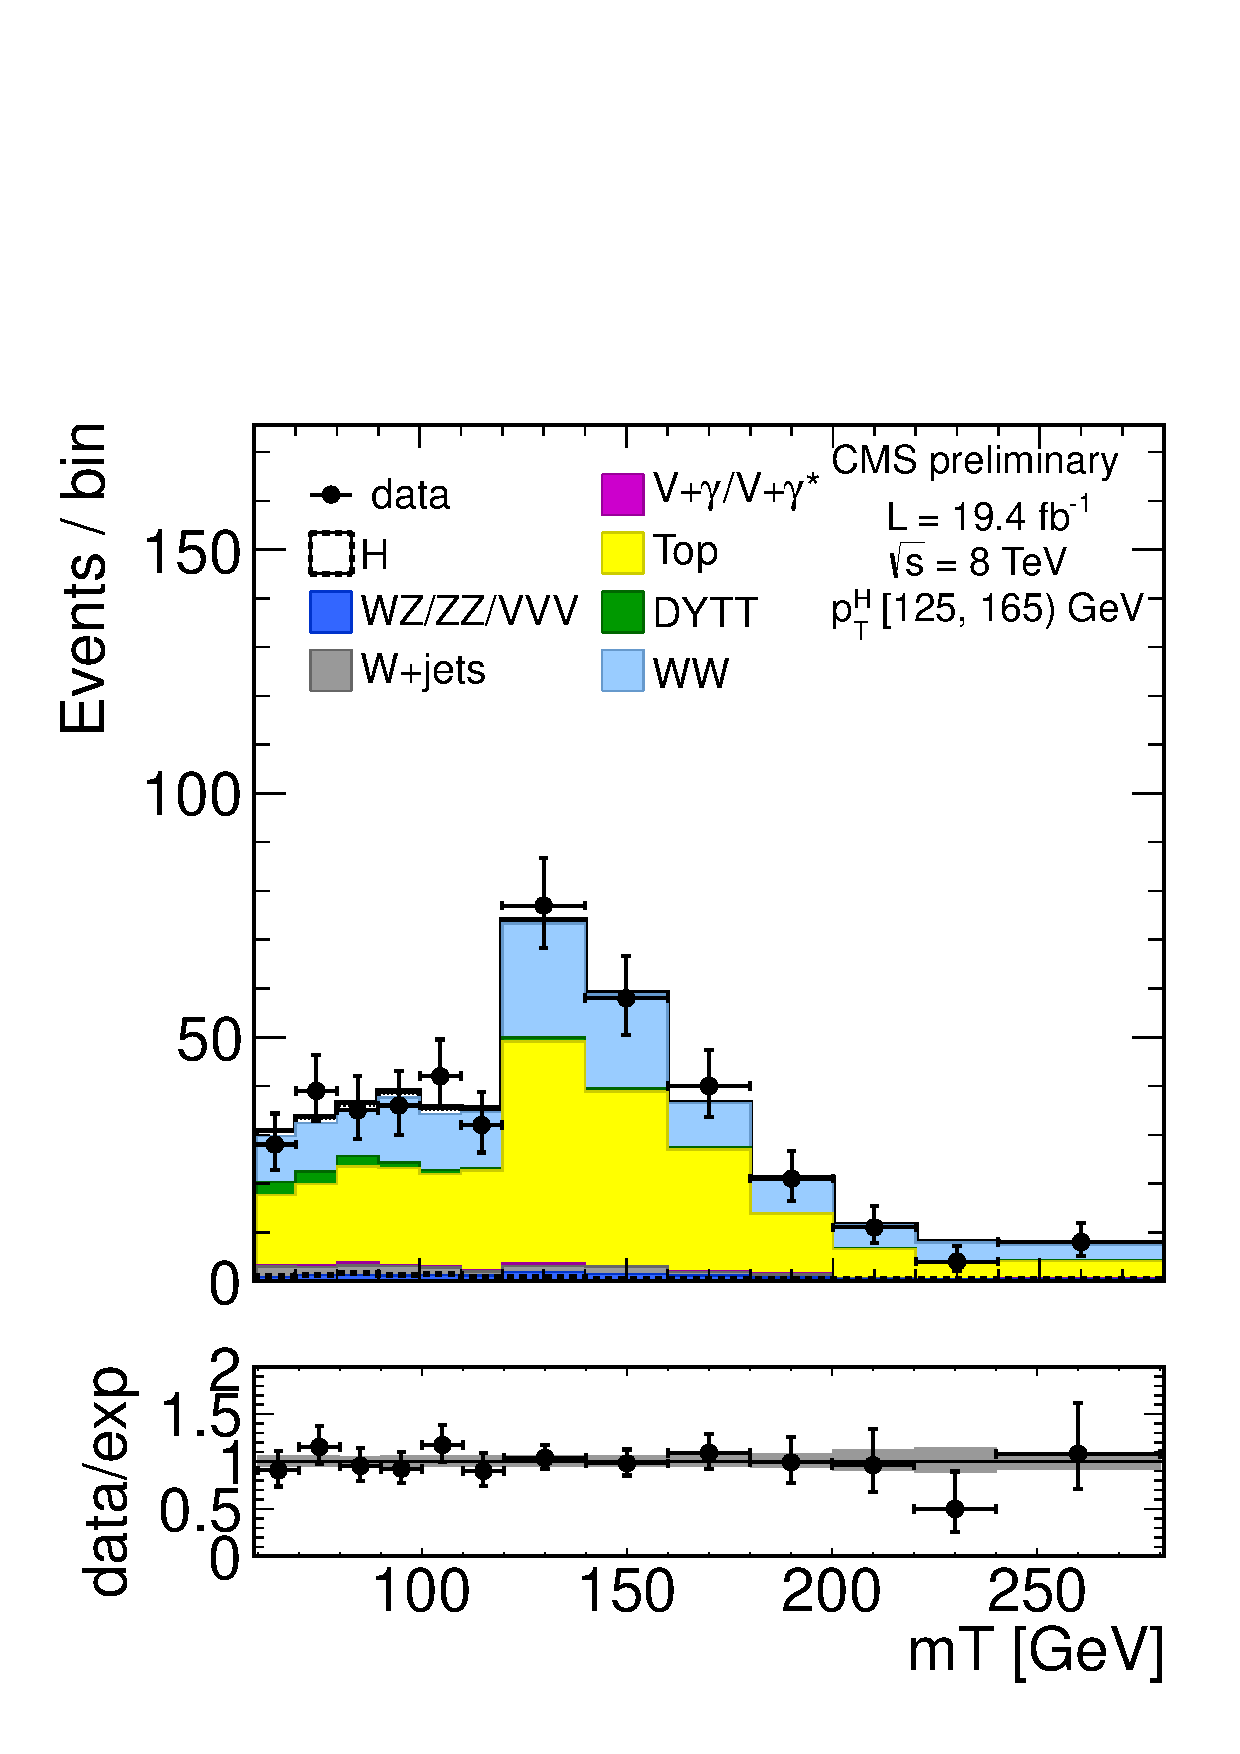
\includegraphics[width=0.31\textwidth]{images/unblinding/mTBin4.pdf}
}
\subfigure{
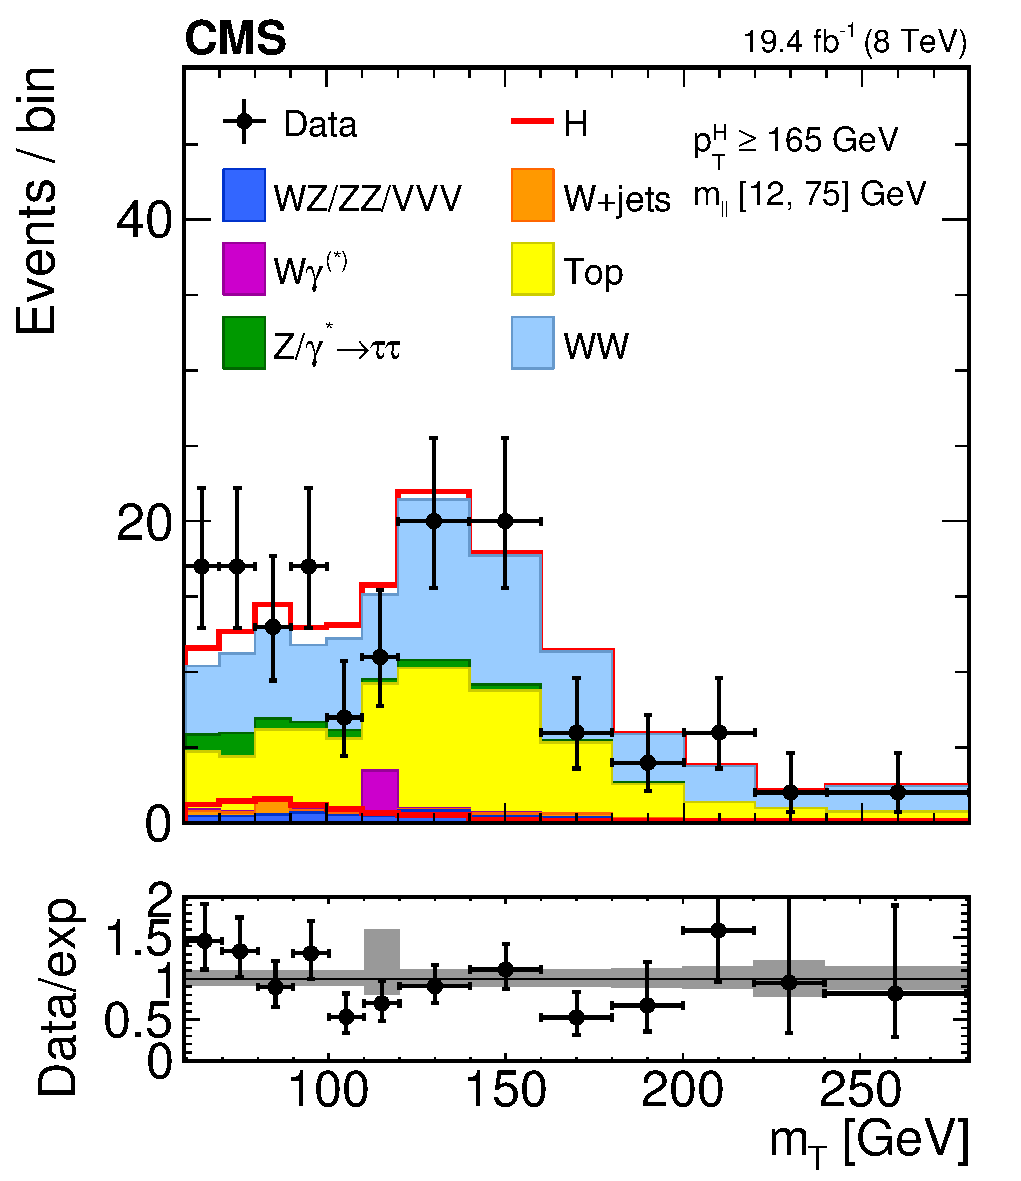
\includegraphics[width=0.31\textwidth]{images/unblinding/mTBin5.pdf}
}
\caption{Distributions of the \mt variable in each of the six \pth{} bins. Background normalizations correspond to the values obtained from the fit. Signal normalization is fixed to the SM expectation. The distributions are shown in an \mll window of [12,75]\GeV in order to emphasize the Higgs boson (H) signal. The signal contribution is shown both stacked on top of the background and superimposed to it. Ratios of the expected and observed event yields in individual bins are shown in the panels below the plots. The uncertainty band shown in the ratio plot corresponds to the envelope of systematic uncertainties after performing the fit to the data.}\label{fig:mTSignalRegion}
\end{figure}

The signal and background yields after the analysis selection are reported in Table \ref{table:yields}.

\begin{table}[htbp]
\small{
\begin{center}{
  \caption{Signal prediction, background estimates and observed number of events in data are shown in each \pth{} bin for the signal after applying the analysis selection requirements. The total uncertainty on the number of events is reported. For signal processes, the yield related to the ggH are shown, separated with respect to the contribution of the other production mechanisms (XH=VBF+VH). The WW process includes both quark and gluon induced contribution, while the Top process takes into account both $\mathrm{t\bar t}$ and tW. }\label{table:yields}
\begin{tabular} {l c c c c c c}
  \hline
$\mathbf{p}_{\rm \mathbf{T}}^{\rm \mathbf{H}} \left[\mathrm{\mathbf{GeV}}\right] $	&	\bf{0-15}	&	\bf{15-45}	&	\bf{45-85}	&	\bf{85-125}	&	\bf{125-165}	&	\bf{165-$\boldsymbol{\infty}$} \\ 	

\hline \hline

ggH	&	$73\pm3$	&	$175\pm5$	&                $59\pm3$	&                $15\pm2$	&                $5.1\pm1.5$	&                $4.9\pm1.4$	\\
XH=VBF+VH	&	$4\pm2$ 	&	$15\pm4$ 	&		 $16\pm4$	&	         $8\pm2$ 	&		 $3.8\pm1.1$ 	&		 $3.0\pm0.8$    \\	
Out-of-fiducial & $9.2\pm0.5$   &       $19.9\pm0.7$    &      $11.4\pm0.6$    &    $4.4\pm0.3$   &     $1.6\pm0.2$   &   $2.4\pm0.2$ \\
Data 	&	2182	 	&         5305	 	&	         3042	 	& 	          1263	 	&	         431	 	& 	          343	 	\\
Total background &  	 $2124\pm128$	 &     $5170\pm321$	 &       $2947\pm293$	 &            $1266\pm175$	 &         $420\pm80$	 &              $336\pm74$	 \\

WW 	& 		$1616\pm107$	 &	 $3172\pm249$	 &	     $865\pm217$	 &	     $421\pm120$	 &	     $125\pm60$	 &		     $161\pm54$	 \\
Top 	&	$184\pm38$	&	                $1199\pm165$	&	                $1741\pm192$	&	                $735\pm125$	&	                $243\pm51$	& 	        $139\pm49$	\\
W+jets 	& $134\pm5$ 	&	         $455\pm10$ 	&	         $174\pm6$ 	&	         $48\pm4$ 	&	         $14\pm3$ 	&	         $9\pm3$ 	\\
WZ+ZZ+VVV & $34\pm4$ 	 &	$107\pm10$ 	&                $71\pm7$ 	&	         $29\pm5$ 	&                $14\pm3$ 	&     $13\pm4$ 	\\
\dytt 	&	$23\pm3$ 	&         $67\pm5$ 	&         $47\pm4$ 	&         $22\pm3$ 	&         $12\pm2$ 	&         $10\pm2$ 	\\
W$\gamma^{(*)}$	& $132\pm49$     &             $170\pm58$    &              $48\pm30$ &                  $12\pm9$ &                  $3\pm3$ &                 $5\pm10$ \\
\hline

\hline
  \end{tabular}
  }
   
  \end{center}
  }
\end{table}


%The signal yield after the fit with data is found to be of $318 \pm 12$ events, to be compared with the expected value of $382 \pm 7$ events.
The spectrum shown in Fig. \ref{fig:pre_unfolding} is obtained after having performed the fit and after the subtraction of the out-of-fiducial signal events, but before undergoing the unfolding procedure. The theoretical distribution after the detector simulation and event reconstruction is also shown for comparison.

\begin{figure}[!h]
\centering
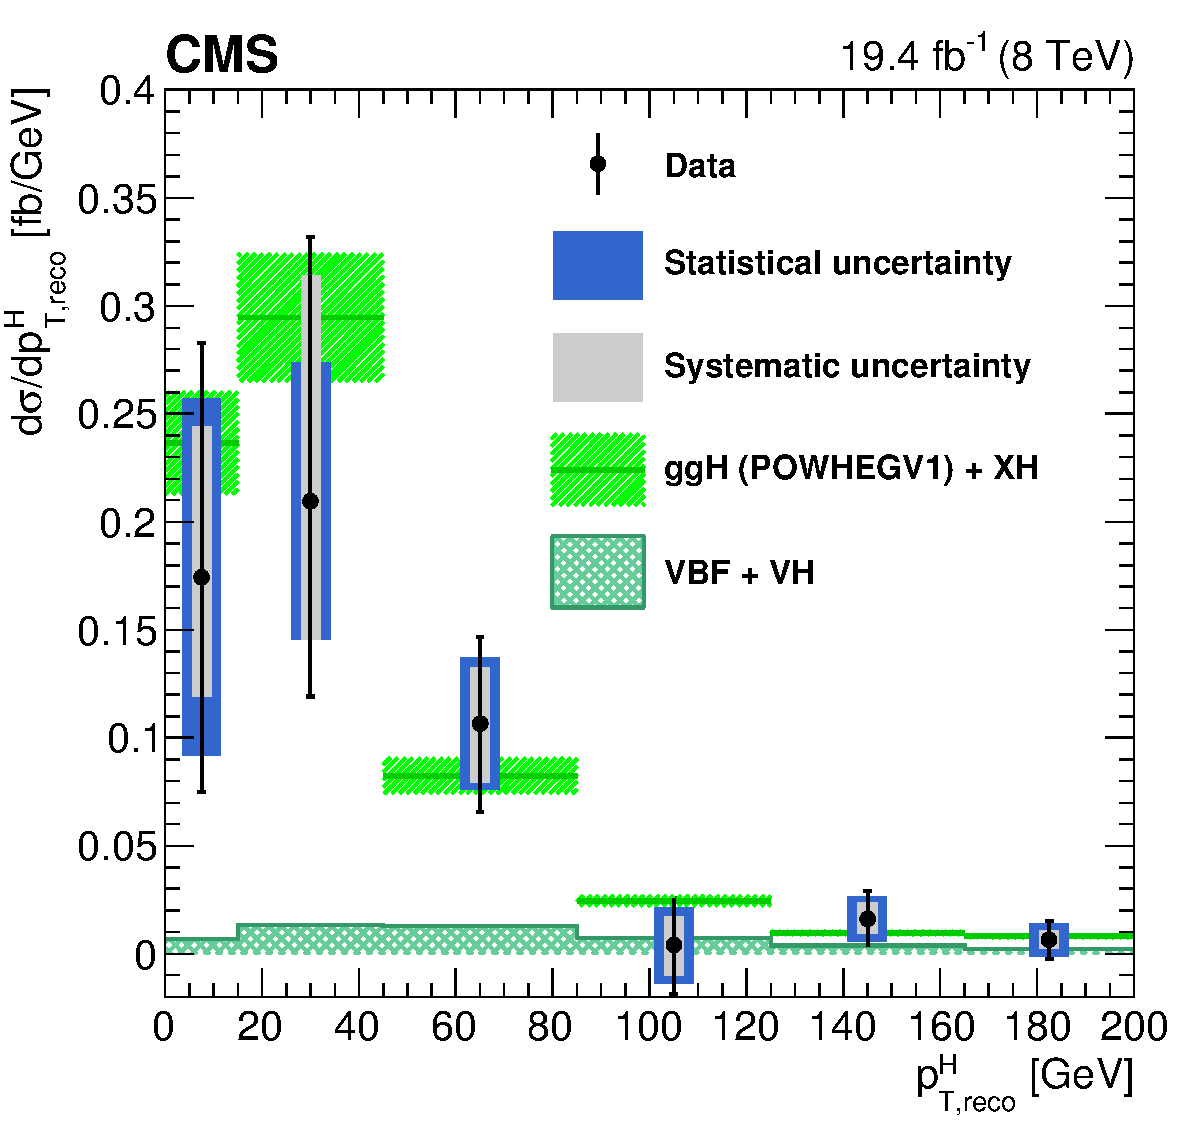
\includegraphics[width=0.8\textwidth]{images/unblinding/pth_reco_paper.pdf}
\caption{Differential Higgs boson production cross section as a function of the reconstructed \pth{}, before applying the unfolding procedure. Data values after the background subtraction are shown together with the statistical and the systematic uncertainties, determined propagating the sources of uncertainty through the fit procedure. The line and dashed area represent the SM theoretical estimates in which the acceptance of the dominant ggH contribution is modelled by \textsc{Powheg V1}. The sub-dominant component of the signal is denoted as XH=VBF+VH, and is shown with the cross filled area separately.}\label{fig:pre_unfolding}
\end{figure}

In order to assess the robustness of the fit, several toy MC samples have been produced, with a statistical accuracy corresponding to the one expected in data. The distribution of the signal strengths extracted in each bin using the toy MC samples and the their pull distributions are shown in Fig.~\ref{fig:pull_fit}. 
\begin{figure}[htb]
\centering
\subfigure[]{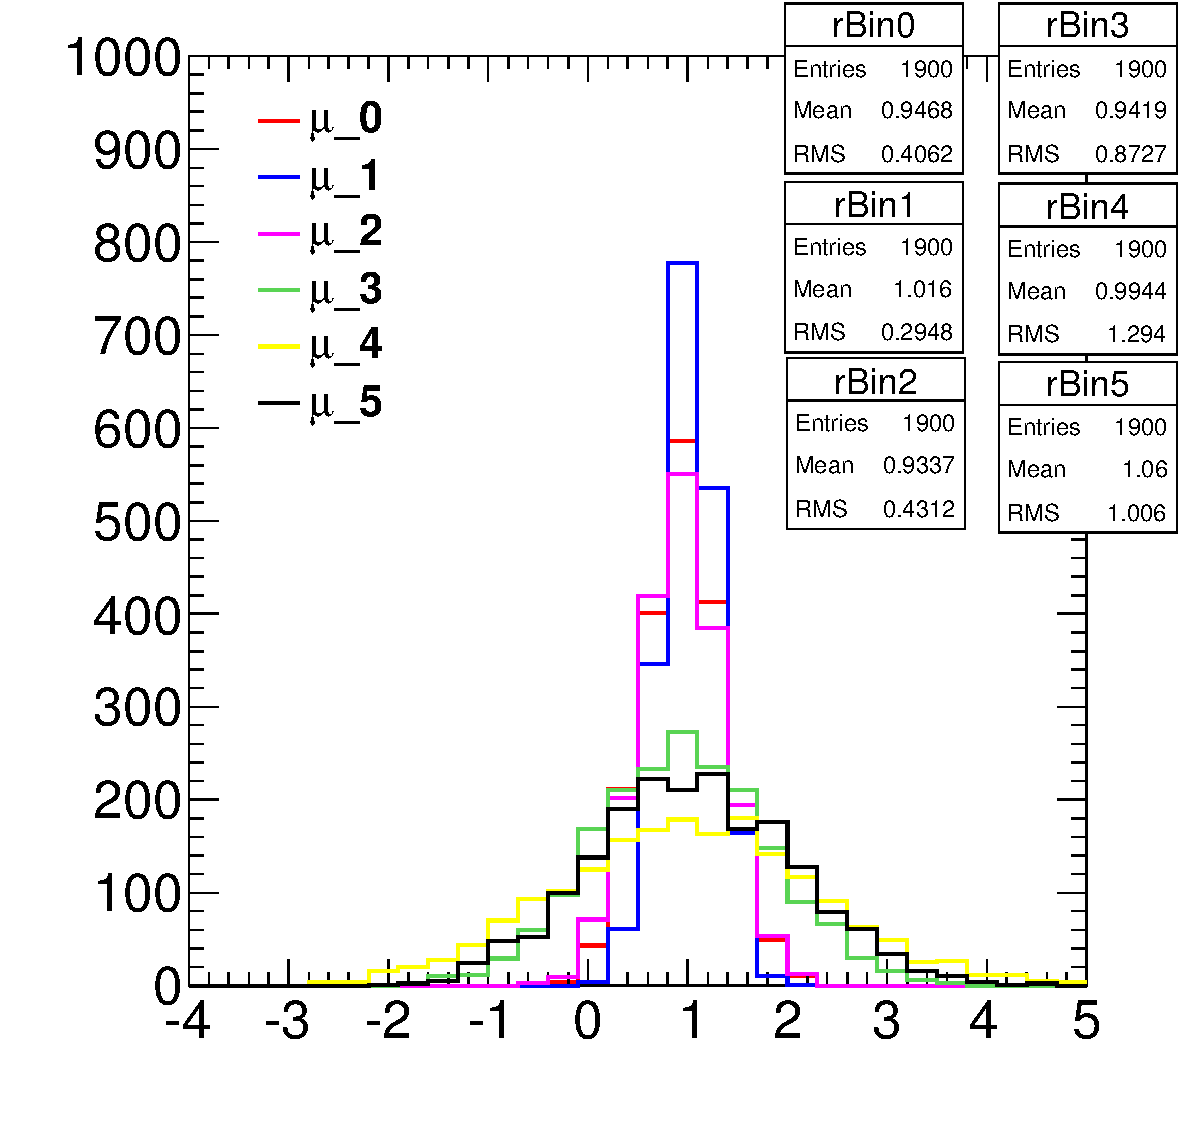
\includegraphics[width=0.45\textwidth]{images/mu_toys.pdf}}
\subfigure[]{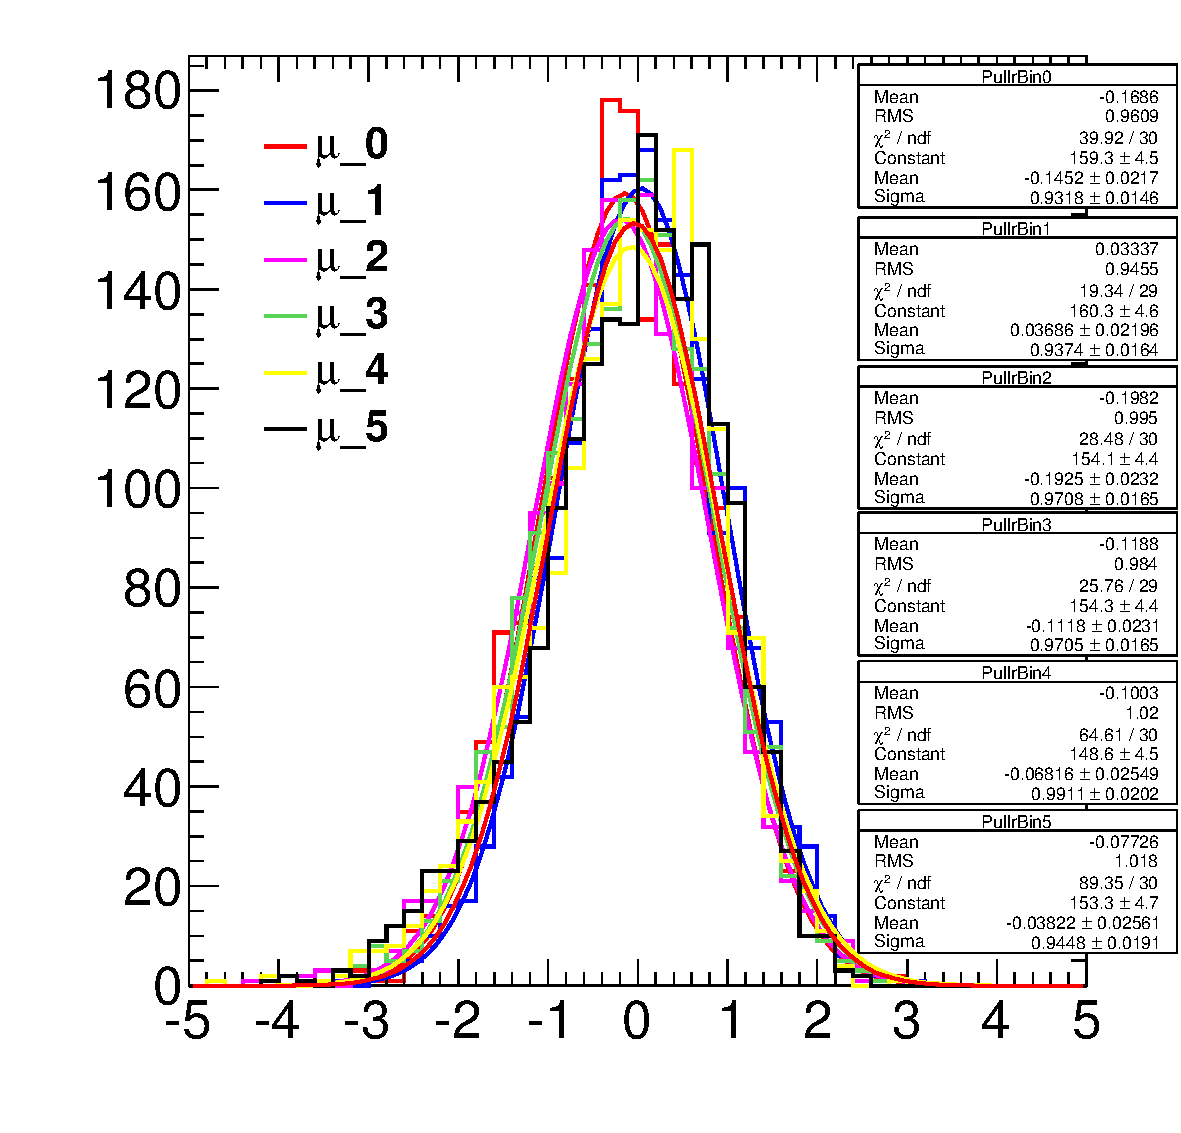
\includegraphics[width=0.45\textwidth]{images/pull_toys.pdf}}
\caption{Signal strength distribution as extracted from the fit of toy MC samples (a). Distribution of the pull of the signal strength parameters (b).\label{fig:pull_fit}}
\end{figure}

%As expected the Top background becomes more important while going to high values of \pth, accordingly to the higher jet multiplicity in that region. The discrepancy between MC prediction and data, especially for low values of Higgs \pt, is due WW background which in this plots is fixed to the MC cross section.

